\documentclass[11pt]{article}

    \usepackage[brazil]{babel}
    \usepackage[utf8]{inputenc}
    \DeclareUnicodeCharacter{2081}{$_1$}
    \DeclareUnicodeCharacter{2082}{$_2$}
    \DeclareUnicodeCharacter{2083}{$_3$}
    \DeclareUnicodeCharacter{2084}{$_4$}
    \DeclareUnicodeCharacter{2085}{$_5$}
    \DeclareUnicodeCharacter{2086}{$_6$}
    \DeclareUnicodeCharacter{2087}{$_7$}
    \DeclareUnicodeCharacter{2088}{$_8$}
    \DeclareUnicodeCharacter{2089}{$_9$}
    \DeclareUnicodeCharacter{2080}{$_0$}

    \usepackage[breakable]{tcolorbox}

    \usepackage{float}
    \usepackage{graphicx, caption}
    \usepackage{xcolor} % Allow colors to be defined
    \usepackage{enumerate} % Needed for markdown enumerations to work
    \usepackage{geometry} % Used to adjust the document margins
    \usepackage{amsmath} % Equations
    \usepackage{amssymb} % Equations
    \usepackage{upquote} % Upright quotes for verbatim code
    \usepackage{eurosym} % defines \euro
    \usepackage{fancyvrb} % verbatim replacement that allows latex
    \usepackage{hyperref}
    \usepackage[inline]{enumitem} 

    % Colors for the hyperref package
    \definecolor{urlcolor}{rgb}{0,.145,.698}
    \definecolor{linkcolor}{rgb}{.71,0.21,0.01}
    \definecolor{citecolor}{rgb}{.12,.54,.11}

    % ANSI colors
    \definecolor{ansi-black}{HTML}{3E424D}
    \definecolor{ansi-black-intense}{HTML}{282C36}
    \definecolor{ansi-red}{HTML}{E75C58}
    \definecolor{ansi-red-intense}{HTML}{B22B31}
    \definecolor{ansi-green}{HTML}{00A250}
    \definecolor{ansi-green-intense}{HTML}{007427}
    \definecolor{ansi-yellow}{HTML}{DDB62B}
    \definecolor{ansi-yellow-intense}{HTML}{B27D12}
    \definecolor{ansi-blue}{HTML}{208FFB}
    \definecolor{ansi-blue-intense}{HTML}{0065CA}
    \definecolor{ansi-magenta}{HTML}{D160C4}
    \definecolor{ansi-magenta-intense}{HTML}{A03196}
    \definecolor{ansi-cyan}{HTML}{60C6C8}
    \definecolor{ansi-cyan-intense}{HTML}{258F8F}
    \definecolor{ansi-white}{HTML}{C5C1B4}
    \definecolor{ansi-white-intense}{HTML}{A1A6B2}
    \definecolor{ansi-default-inverse-fg}{HTML}{FFFFFF}
    \definecolor{ansi-default-inverse-bg}{HTML}{000000}

    \providecommand{\tightlist}{%
      \setlength{\itemsep}{0pt}\setlength{\parskip}{0pt}}
    \DefineVerbatimEnvironment{Highlighting}{Verbatim}{commandchars=\\\{\}}
    \newenvironment{Shaded}{}{}
    \newcommand{\KeywordTok}[1]{\textcolor[rgb]{0.00,0.44,0.13}{\textbf{{#1}}}}
    \newcommand{\DataTypeTok}[1]{\textcolor[rgb]{0.56,0.13,0.00}{{#1}}}
    \newcommand{\DecValTok}[1]{\textcolor[rgb]{0.25,0.63,0.44}{{#1}}}
    \newcommand{\BaseNTok}[1]{\textcolor[rgb]{0.25,0.63,0.44}{{#1}}}
    \newcommand{\FloatTok}[1]{\textcolor[rgb]{0.25,0.63,0.44}{{#1}}}
    \newcommand{\CharTok}[1]{\textcolor[rgb]{0.25,0.44,0.63}{{#1}}}
    \newcommand{\StringTok}[1]{\textcolor[rgb]{0.25,0.44,0.63}{{#1}}}
    \newcommand{\CommentTok}[1]{\textcolor[rgb]{0.38,0.63,0.69}{\textit{{#1}}}}
    \newcommand{\OtherTok}[1]{\textcolor[rgb]{0.00,0.44,0.13}{{#1}}}
    \newcommand{\AlertTok}[1]{\textcolor[rgb]{1.00,0.00,0.00}{\textbf{{#1}}}}
    \newcommand{\FunctionTok}[1]{\textcolor[rgb]{0.02,0.16,0.49}{{#1}}}
    \newcommand{\RegionMarkerTok}[1]{{#1}}
    \newcommand{\ErrorTok}[1]{\textcolor[rgb]{1.00,0.00,0.00}{\textbf{{#1}}}}
    \newcommand{\NormalTok}[1]{{#1}}
    
    % Additional commands for more recent versions of Pandoc
    \newcommand{\ConstantTok}[1]{\textcolor[rgb]{0.53,0.00,0.00}{{#1}}}
    \newcommand{\SpecialCharTok}[1]{\textcolor[rgb]{0.25,0.44,0.63}{{#1}}}
    \newcommand{\VerbatimStringTok}[1]{\textcolor[rgb]{0.25,0.44,0.63}{{#1}}}
    \newcommand{\SpecialStringTok}[1]{\textcolor[rgb]{0.73,0.40,0.53}{{#1}}}
    \newcommand{\ImportTok}[1]{{#1}}
    \newcommand{\DocumentationTok}[1]{\textcolor[rgb]{0.73,0.13,0.13}{\textit{{#1}}}}
    \newcommand{\AnnotationTok}[1]{\textcolor[rgb]{0.38,0.63,0.69}{\textbf{\textit{{#1}}}}}
    \newcommand{\CommentVarTok}[1]{\textcolor[rgb]{0.38,0.63,0.69}{\textbf{\textit{{#1}}}}}
    \newcommand{\VariableTok}[1]{\textcolor[rgb]{0.10,0.09,0.49}{{#1}}}
    \newcommand{\ControlFlowTok}[1]{\textcolor[rgb]{0.00,0.44,0.13}{\textbf{{#1}}}}
    \newcommand{\OperatorTok}[1]{\textcolor[rgb]{0.40,0.40,0.40}{{#1}}}
    \newcommand{\BuiltInTok}[1]{{#1}}
    \newcommand{\ExtensionTok}[1]{{#1}}
    \newcommand{\PreprocessorTok}[1]{\textcolor[rgb]{0.74,0.48,0.00}{{#1}}}
    \newcommand{\AttributeTok}[1]{\textcolor[rgb]{0.49,0.56,0.16}{{#1}}}
    \newcommand{\InformationTok}[1]{\textcolor[rgb]{0.38,0.63,0.69}{\textbf{\textit{{#1}}}}}
    \newcommand{\WarningTok}[1]{\textcolor[rgb]{0.38,0.63,0.69}{\textbf{\textit{{#1}}}}}
    
    
    \def\br{\hspace*{\fill} \\* }
    \def\gt{>}
    \def\lt{<}
    \let\Oldtex\TeX
    \let\Oldlatex\LaTeX
    \renewcommand{\TeX}{\textrm{\Oldtex}}
    \renewcommand{\LaTeX}{\textrm{\Oldlatex}}
    % Document parameters
    % Document title
    \title{Interações entre proteínas e entre domínios}
    \author{Lucas Machado Moschen}
    
\makeatletter
\def\PY@reset{\let\PY@it=\relax \let\PY@bf=\relax%
    \let\PY@ul=\relax \let\PY@tc=\relax%
    \let\PY@bc=\relax \let\PY@ff=\relax}
\def\PY@tok#1{\csname PY@tok@#1\endcsname}
\def\PY@toks#1+{\ifx\relax#1\empty\else%
    \PY@tok{#1}\expandafter\PY@toks\fi}
\def\PY@do#1{\PY@bc{\PY@tc{\PY@ul{%
    \PY@it{\PY@bf{\PY@ff{#1}}}}}}}
\def\PY#1#2{\PY@reset\PY@toks#1+\relax+\PY@do{#2}}

\expandafter\def\csname PY@tok@w\endcsname{\def\PY@tc##1{\textcolor[rgb]{0.73,0.73,0.73}{##1}}}
\expandafter\def\csname PY@tok@c\endcsname{\let\PY@it=\textit\def\PY@tc##1{\textcolor[rgb]{0.25,0.50,0.50}{##1}}}
\expandafter\def\csname PY@tok@cp\endcsname{\def\PY@tc##1{\textcolor[rgb]{0.74,0.48,0.00}{##1}}}
\expandafter\def\csname PY@tok@k\endcsname{\let\PY@bf=\textbf\def\PY@tc##1{\textcolor[rgb]{0.00,0.50,0.00}{##1}}}
\expandafter\def\csname PY@tok@kp\endcsname{\def\PY@tc##1{\textcolor[rgb]{0.00,0.50,0.00}{##1}}}
\expandafter\def\csname PY@tok@kt\endcsname{\def\PY@tc##1{\textcolor[rgb]{0.69,0.00,0.25}{##1}}}
\expandafter\def\csname PY@tok@o\endcsname{\def\PY@tc##1{\textcolor[rgb]{0.40,0.40,0.40}{##1}}}
\expandafter\def\csname PY@tok@ow\endcsname{\let\PY@bf=\textbf\def\PY@tc##1{\textcolor[rgb]{0.67,0.13,1.00}{##1}}}
\expandafter\def\csname PY@tok@nb\endcsname{\def\PY@tc##1{\textcolor[rgb]{0.00,0.50,0.00}{##1}}}
\expandafter\def\csname PY@tok@nf\endcsname{\def\PY@tc##1{\textcolor[rgb]{0.00,0.00,1.00}{##1}}}
\expandafter\def\csname PY@tok@nc\endcsname{\let\PY@bf=\textbf\def\PY@tc##1{\textcolor[rgb]{0.00,0.00,1.00}{##1}}}
\expandafter\def\csname PY@tok@nn\endcsname{\let\PY@bf=\textbf\def\PY@tc##1{\textcolor[rgb]{0.00,0.00,1.00}{##1}}}
\expandafter\def\csname PY@tok@ne\endcsname{\let\PY@bf=\textbf\def\PY@tc##1{\textcolor[rgb]{0.82,0.25,0.23}{##1}}}
\expandafter\def\csname PY@tok@nv\endcsname{\def\PY@tc##1{\textcolor[rgb]{0.10,0.09,0.49}{##1}}}
\expandafter\def\csname PY@tok@no\endcsname{\def\PY@tc##1{\textcolor[rgb]{0.53,0.00,0.00}{##1}}}
\expandafter\def\csname PY@tok@nl\endcsname{\def\PY@tc##1{\textcolor[rgb]{0.63,0.63,0.00}{##1}}}
\expandafter\def\csname PY@tok@ni\endcsname{\let\PY@bf=\textbf\def\PY@tc##1{\textcolor[rgb]{0.60,0.60,0.60}{##1}}}
\expandafter\def\csname PY@tok@na\endcsname{\def\PY@tc##1{\textcolor[rgb]{0.49,0.56,0.16}{##1}}}
\expandafter\def\csname PY@tok@nt\endcsname{\let\PY@bf=\textbf\def\PY@tc##1{\textcolor[rgb]{0.00,0.50,0.00}{##1}}}
\expandafter\def\csname PY@tok@nd\endcsname{\def\PY@tc##1{\textcolor[rgb]{0.67,0.13,1.00}{##1}}}
\expandafter\def\csname PY@tok@s\endcsname{\def\PY@tc##1{\textcolor[rgb]{0.73,0.13,0.13}{##1}}}
\expandafter\def\csname PY@tok@sd\endcsname{\let\PY@it=\textit\def\PY@tc##1{\textcolor[rgb]{0.73,0.13,0.13}{##1}}}
\expandafter\def\csname PY@tok@si\endcsname{\let\PY@bf=\textbf\def\PY@tc##1{\textcolor[rgb]{0.73,0.40,0.53}{##1}}}
\expandafter\def\csname PY@tok@se\endcsname{\let\PY@bf=\textbf\def\PY@tc##1{\textcolor[rgb]{0.73,0.40,0.13}{##1}}}
\expandafter\def\csname PY@tok@sr\endcsname{\def\PY@tc##1{\textcolor[rgb]{0.73,0.40,0.53}{##1}}}
\expandafter\def\csname PY@tok@ss\endcsname{\def\PY@tc##1{\textcolor[rgb]{0.10,0.09,0.49}{##1}}}
\expandafter\def\csname PY@tok@sx\endcsname{\def\PY@tc##1{\textcolor[rgb]{0.00,0.50,0.00}{##1}}}
\expandafter\def\csname PY@tok@m\endcsname{\def\PY@tc##1{\textcolor[rgb]{0.40,0.40,0.40}{##1}}}
\expandafter\def\csname PY@tok@gh\endcsname{\let\PY@bf=\textbf\def\PY@tc##1{\textcolor[rgb]{0.00,0.00,0.50}{##1}}}
\expandafter\def\csname PY@tok@gu\endcsname{\let\PY@bf=\textbf\def\PY@tc##1{\textcolor[rgb]{0.50,0.00,0.50}{##1}}}
\expandafter\def\csname PY@tok@gd\endcsname{\def\PY@tc##1{\textcolor[rgb]{0.63,0.00,0.00}{##1}}}
\expandafter\def\csname PY@tok@gi\endcsname{\def\PY@tc##1{\textcolor[rgb]{0.00,0.63,0.00}{##1}}}
\expandafter\def\csname PY@tok@gr\endcsname{\def\PY@tc##1{\textcolor[rgb]{1.00,0.00,0.00}{##1}}}
\expandafter\def\csname PY@tok@ge\endcsname{\let\PY@it=\textit}
\expandafter\def\csname PY@tok@gs\endcsname{\let\PY@bf=\textbf}
\expandafter\def\csname PY@tok@gp\endcsname{\let\PY@bf=\textbf\def\PY@tc##1{\textcolor[rgb]{0.00,0.00,0.50}{##1}}}
\expandafter\def\csname PY@tok@go\endcsname{\def\PY@tc##1{\textcolor[rgb]{0.53,0.53,0.53}{##1}}}
\expandafter\def\csname PY@tok@gt\endcsname{\def\PY@tc##1{\textcolor[rgb]{0.00,0.27,0.87}{##1}}}
\expandafter\def\csname PY@tok@err\endcsname{\def\PY@bc##1{\setlength{\fboxsep}{0pt}\fcolorbox[rgb]{1.00,0.00,0.00}{1,1,1}{\strut ##1}}}
\expandafter\def\csname PY@tok@kc\endcsname{\let\PY@bf=\textbf\def\PY@tc##1{\textcolor[rgb]{0.00,0.50,0.00}{##1}}}
\expandafter\def\csname PY@tok@kd\endcsname{\let\PY@bf=\textbf\def\PY@tc##1{\textcolor[rgb]{0.00,0.50,0.00}{##1}}}
\expandafter\def\csname PY@tok@kn\endcsname{\let\PY@bf=\textbf\def\PY@tc##1{\textcolor[rgb]{0.00,0.50,0.00}{##1}}}
\expandafter\def\csname PY@tok@kr\endcsname{\let\PY@bf=\textbf\def\PY@tc##1{\textcolor[rgb]{0.00,0.50,0.00}{##1}}}
\expandafter\def\csname PY@tok@bp\endcsname{\def\PY@tc##1{\textcolor[rgb]{0.00,0.50,0.00}{##1}}}
\expandafter\def\csname PY@tok@fm\endcsname{\def\PY@tc##1{\textcolor[rgb]{0.00,0.00,1.00}{##1}}}
\expandafter\def\csname PY@tok@vc\endcsname{\def\PY@tc##1{\textcolor[rgb]{0.10,0.09,0.49}{##1}}}
\expandafter\def\csname PY@tok@vg\endcsname{\def\PY@tc##1{\textcolor[rgb]{0.10,0.09,0.49}{##1}}}
\expandafter\def\csname PY@tok@vi\endcsname{\def\PY@tc##1{\textcolor[rgb]{0.10,0.09,0.49}{##1}}}
\expandafter\def\csname PY@tok@vm\endcsname{\def\PY@tc##1{\textcolor[rgb]{0.10,0.09,0.49}{##1}}}
\expandafter\def\csname PY@tok@sa\endcsname{\def\PY@tc##1{\textcolor[rgb]{0.73,0.13,0.13}{##1}}}
\expandafter\def\csname PY@tok@sb\endcsname{\def\PY@tc##1{\textcolor[rgb]{0.73,0.13,0.13}{##1}}}
\expandafter\def\csname PY@tok@sc\endcsname{\def\PY@tc##1{\textcolor[rgb]{0.73,0.13,0.13}{##1}}}
\expandafter\def\csname PY@tok@dl\endcsname{\def\PY@tc##1{\textcolor[rgb]{0.73,0.13,0.13}{##1}}}
\expandafter\def\csname PY@tok@s2\endcsname{\def\PY@tc##1{\textcolor[rgb]{0.73,0.13,0.13}{##1}}}
\expandafter\def\csname PY@tok@sh\endcsname{\def\PY@tc##1{\textcolor[rgb]{0.73,0.13,0.13}{##1}}}
\expandafter\def\csname PY@tok@s1\endcsname{\def\PY@tc##1{\textcolor[rgb]{0.73,0.13,0.13}{##1}}}
\expandafter\def\csname PY@tok@mb\endcsname{\def\PY@tc##1{\textcolor[rgb]{0.40,0.40,0.40}{##1}}}
\expandafter\def\csname PY@tok@mf\endcsname{\def\PY@tc##1{\textcolor[rgb]{0.40,0.40,0.40}{##1}}}
\expandafter\def\csname PY@tok@mh\endcsname{\def\PY@tc##1{\textcolor[rgb]{0.40,0.40,0.40}{##1}}}
\expandafter\def\csname PY@tok@mi\endcsname{\def\PY@tc##1{\textcolor[rgb]{0.40,0.40,0.40}{##1}}}
\expandafter\def\csname PY@tok@il\endcsname{\def\PY@tc##1{\textcolor[rgb]{0.40,0.40,0.40}{##1}}}
\expandafter\def\csname PY@tok@mo\endcsname{\def\PY@tc##1{\textcolor[rgb]{0.40,0.40,0.40}{##1}}}
\expandafter\def\csname PY@tok@ch\endcsname{\let\PY@it=\textit\def\PY@tc##1{\textcolor[rgb]{0.25,0.50,0.50}{##1}}}
\expandafter\def\csname PY@tok@cm\endcsname{\let\PY@it=\textit\def\PY@tc##1{\textcolor[rgb]{0.25,0.50,0.50}{##1}}}
\expandafter\def\csname PY@tok@cpf\endcsname{\let\PY@it=\textit\def\PY@tc##1{\textcolor[rgb]{0.25,0.50,0.50}{##1}}}
\expandafter\def\csname PY@tok@c1\endcsname{\let\PY@it=\textit\def\PY@tc##1{\textcolor[rgb]{0.25,0.50,0.50}{##1}}}
\expandafter\def\csname PY@tok@cs\endcsname{\let\PY@it=\textit\def\PY@tc##1{\textcolor[rgb]{0.25,0.50,0.50}{##1}}}

\def\PYZbs{\char`\\}
\def\PYZus{\char`\_}
\def\PYZob{\char`\{}
\def\PYZcb{\char`\}}
\def\PYZca{\char`\^}
\def\PYZam{\char`\&}
\def\PYZlt{\char`\<}
\def\PYZgt{\char`\>}
\def\PYZsh{\char`\#}
\def\PYZpc{\char`\%}
\def\PYZdl{\char`\$}
\def\PYZhy{\char`\-}
\def\PYZsq{\char`\'}
\def\PYZdq{\char`\"}
\def\PYZti{\char`\~}
% for compatibility with earlier versions
\def\PYZat{@}
\def\PYZlb{[}
\def\PYZrb{]}
\makeatother

    \makeatletter
        \newbox\Wrappedcontinuationbox 
        \newbox\Wrappedvisiblespacebox 
        \newcommand*\Wrappedvisiblespace {\textcolor{red}{\textvisiblespace}} 
        \newcommand*\Wrappedcontinuationsymbol {\textcolor{red}{\llap{\tiny$\m@th\hookrightarrow$}}} 
        \newcommand*\Wrappedcontinuationindent {3ex } 
        \newcommand*\Wrappedafterbreak {\kern\Wrappedcontinuationindent\copy\Wrappedcontinuationbox} 
        \newcommand*\Wrappedbreaksatspecials {% 
            \def\PYGZus{\discretionary{\char`\_}{\Wrappedafterbreak}{\char`\_}}% 
            \def\PYGZob{\discretionary{}{\Wrappedafterbreak\char`\{}{\char`\{}}% 
            \def\PYGZcb{\discretionary{\char`\}}{\Wrappedafterbreak}{\char`\}}}% 
            \def\PYGZca{\discretionary{\char`\^}{\Wrappedafterbreak}{\char`\^}}% 
            \def\PYGZam{\discretionary{\char`\&}{\Wrappedafterbreak}{\char`\&}}% 
            \def\PYGZlt{\discretionary{}{\Wrappedafterbreak\char`\<}{\char`\<}}% 
            \def\PYGZgt{\discretionary{\char`\>}{\Wrappedafterbreak}{\char`\>}}% 
            \def\PYGZsh{\discretionary{}{\Wrappedafterbreak\char`\#}{\char`\#}}% 
            \def\PYGZpc{\discretionary{}{\Wrappedafterbreak\char`\%}{\char`\%}}% 
            \def\PYGZdl{\discretionary{}{\Wrappedafterbreak\char`\$}{\char`\$}}% 
            \def\PYGZhy{\discretionary{\char`\-}{\Wrappedafterbreak}{\char`\-}}% 
            \def\PYGZsq{\discretionary{}{\Wrappedafterbreak\textquotesingle}{\textquotesingle}}% 
            \def\PYGZdq{\discretionary{}{\Wrappedafterbreak\char`\"}{\char`\"}}% 
            \def\PYGZti{\discretionary{\char`\~}{\Wrappedafterbreak}{\char`\~}}% 
        } 
        \newcommand*\Wrappedbreaksatpunct {% 
            \lccode`\~`\.\lowercase{\def~}{\discretionary{\hbox{\char`\.}}{\Wrappedafterbreak}{\hbox{\char`\.}}}% 
            \lccode`\~`\,\lowercase{\def~}{\discretionary{\hbox{\char`\,}}{\Wrappedafterbreak}{\hbox{\char`\,}}}% 
            \lccode`\~`\;\lowercase{\def~}{\discretionary{\hbox{\char`\;}}{\Wrappedafterbreak}{\hbox{\char`\;}}}% 
            \lccode`\~`\:\lowercase{\def~}{\discretionary{\hbox{\char`\:}}{\Wrappedafterbreak}{\hbox{\char`\:}}}% 
            \lccode`\~`\?\lowercase{\def~}{\discretionary{\hbox{\char`\?}}{\Wrappedafterbreak}{\hbox{\char`\?}}}% 
            \lccode`\~`\!\lowercase{\def~}{\discretionary{\hbox{\char`\!}}{\Wrappedafterbreak}{\hbox{\char`\!}}}% 
            \lccode`\~`\/\lowercase{\def~}{\discretionary{\hbox{\char`\/}}{\Wrappedafterbreak}{\hbox{\char`\/}}}% 
            \catcode`\.\active
            \catcode`\,\active 
            \catcode`\;\active
            \catcode`\:\active
            \catcode`\?\active
            \catcode`\!\active
            \catcode`\/\active 
            \lccode`\~`\~ 	
        }
    \makeatother

    \let\OriginalVerbatim=\Verbatim
    \makeatletter
    \renewcommand{\Verbatim}[1][1]{%
        %\parskip\z@skip
        \sbox\Wrappedcontinuationbox {\Wrappedcontinuationsymbol}%
        \sbox\Wrappedvisiblespacebox {\FV@SetupFont\Wrappedvisiblespace}%
        \def\FancyVerbFormatLine ##1{\hsize\linewidth
            \vtop{\raggedright\hyphenpenalty\z@\exhyphenpenalty\z@
                \doublehyphendemerits\z@\finalhyphendemerits\z@
                \strut ##1\strut}%
        }
        \def\FV@Space {%
            \nobreak\hskip\z@ plus\fontdimen3\font minus\fontdimen4\font
            \discretionary{\copy\Wrappedvisiblespacebox}{\Wrappedafterbreak}
            {\kern\fontdimen2\font}%
        }%
        \Wrappedbreaksatspecials
        \OriginalVerbatim[#1,codes*=\Wrappedbreaksatpunct]%
    }
    \makeatother

    \definecolor{incolor}{HTML}{303F9F}
    \definecolor{outcolor}{HTML}{D84315}
    \definecolor{cellborder}{HTML}{CFCFCF}
    \definecolor{cellbackground}{HTML}{F7F7F7}
    
    \makeatletter
    \newcommand{\boxspacing}{\kern\kvtcb@left@rule\kern\kvtcb@boxsep}
    \makeatother
    \newcommand{\prompt}[4]{
        \ttfamily\llap{{\color{#2}[#3]:\hspace{3pt}#4}}\vspace{-\baselineskip}
    }
        
    \sloppy 
    \hypersetup{
      breaklinks=true,  % so long urls are correctly broken across lines
      colorlinks=true,
      urlcolor=urlcolor,
      linkcolor=linkcolor,
      citecolor=citecolor,
      }
    
    \geometry{verbose,tmargin=1in,bmargin=1in,lmargin=1in,rmargin=1in}

\begin{document}
    
    \maketitle
    
\textbf{Professor:} Luciano Guimarães de Castro

\begin{abstract}
   Um estudo sobre como redes de interação proteína-proteína podem inferir
interações domínio-domínio utilizando uma abordagem de programação
linear e inteira. Essa abordagem é baseada no conceito de parcimônia, isto é, dados modelos diferentes que representem um fenômeno, se não haver evidência, escolhemos o modelo mais simples.
\end{abstract}


\tableofcontents

\section{Introdução}
\label{intro}

Proteínas são macromoléculas formadas por cadeias de aminoácidos. Elas
são construídas em formato modular, compostas por domínios, que são
unidades da proteína funcionais ou estruturais independentes do resto.
Muitas são construídas por dois ou mais domínios dentro de um repertório
relativamente pequeno, como na Figura \ref{fig1:p-d}. O que variam são as combinações e a ordem de
disposição. Frequentemente, os domínios individuais têm funções
específicas, como catalisar uma reação ou ligação de uma molécula
particular \cite{livro, embl}.

\begin{figure}
    \centering
    \includegraphics[width=0.8\textwidth]{images/figure-protein-domains.png}
    \caption{Representação da proteína citoplasmática Nck com seus três
    domínios SH3 e outro domínio SH2. Cada um desses domínios possui um
    parceiro de ligação em outras proteínas. Disponível em EMBL-EBI.}
    \label{fig1:p-d}
\end{figure}

Proteínas interagem umas com as outras nas células e o conjunto dessas
interações é chamado de Rede de Interações Proteína-Proteína (Rede PPI), como
na Figura \ref{fig2:ppi}. 
Matematicamente, representamo elas como um grafo (direcionado ou não
direcionado) cujos nós são as proteínas e cujas arestas são as
interações entre as proteínas, verificadas experimentalmente. Uma rede
PPI é a base molecular do desenvolvimento e do funcionamento dos
organismos. Seu entendimento é essencial, tanto para a compreensão de
estados normais e doentes de células, quanto para o desenvolvimento de
drogas. Ela pode ser construída para descrever uma série de informações,
como, por exemplo, proteínas que estão na mesma regiões ao mesmo tempo;
proteínas que são correguladas; proteínas que estão envolvidas com
alguma função biológica; entre outras \cite{embl}. Em particular, o tópico
de minha possível dissertação vai nesse sentido e, por esse motivo, foi
o tema escolhido.

\begin{figure}
    \centering
    \includegraphics[width=\textwidth]{images/ppi-network.png}
    \caption{Exemplo de rede PPI usando NetworkAnalysist. Desenvolvido por \href{https://www.researchgate.net/figure/An-overview-of-the-PPI-network-The-PPI-network-was-generated-using-NetworkAnalyst-Red_fig5_323136513}{Wei
    Zhong, et al.}}
    \label{fig2:ppi}
\end{figure}

Como as interações entre proteínas geralmente ocorrem via domínios ao
invés de toda a molécula, entender como os domínios interagem entre si
pode facilitar a obtenção de redes PPI mais completas, com menor custo e
tempo. Por esse motivo, predizer interações entre domínios (DDI) é um
passo importante para a predição de PPI. Chamamos esse problema de
problema de interação domínio-domínio (DDIP).

\section{O problema de interação domínio-domínio (DDIP)}
\label{ddip}

Denotamos uma rede PPI conhecida por um grafo não direcionado
\(\mathcal{N} = (\mathcal{P}, \mathcal{E})\), em que \(\mathcal{P}\) é o
conjunto de proteínas e \(\mathcal{E}\) é o conjunto de pares de
proteínas que interagem, dado algum experimento. Para cada proteína
\(P \in \mathcal{P}\), supomos conhecidos seus domínios \(D_P\) e
definimos
\(\mathcal{D} = \{\{d_1, d_2\} : d_1 \in D_{P_1}, d_2 \in D_{P_2}, \text{ e } \{P_1, P_2\} \in \mathcal{E}\}\),
isto é, o conjunto dos pares (não ordenados) de possíveis interações
domínio domínio. Então, queremos inferir, para cada
\(I = \{P_1, P_2\} \in \mathcal{E}\), quais pares de domínios distintos
em \(D_{P_1}\) e \(D_{P_2}\) explicam a interação entre as proteínas
\cite{livro}.

Vamos assumir que as interações domínio-domínio são conservadas entre as
várias interações entre proteínas, isto é, elas tendem a repetir em
diversos contextos. Também supomos que a interação entre proteínas
evolui de forma parcimoniosa e que o conjunto DDI é bem aproximado pelo
menor conjunto de interações necessárias para explicar a rede PPI, ou
seja, sabemos que as relações domínio-domínio influenciam fortemente as
relações proteína-proteína e utilizamos um método baseado em parcimônia
para explicar essa inferência. O objetivo será, portanto, minimizar o
número de interações domínio-domínio que justifiquem a interação entre
proteínas observada na rede \cite{guimaraes}.

Seja \(\mathcal{B}\) um grafo bipartido não direcionado com dois
conjuntos independentes: \(\mathcal{P}^2 = \mathcal{E}\) (conjunto dos
pares de interações proteína-proteína) e \(\mathcal{D}\) (pares de
domínios), em que um elemento \(\{P_1, P_2\} \in \mathcal{P}^2\) é
ligado a \(\{d_1, d_2\} \in \mathcal{D}\) se \(d_1 \in D_{P_1}\) e
\(d_2 \in D_{P_2}\).

\begin{figure}
    \centering
    \includegraphics[width=0.9\textwidth]{images/ddi-ppi-example.png}
    \caption{Exemplo simplificado de rede PPI com respectivos domínios e a
    construção do grafo bipartido correspondente.}
    \label{fig3:example}
\end{figure}

{\bf Definição (Cobertura):} Um conjunto \(S \subset \mathcal{D}\) é cobertura
DDI se cada nó em \(\mathcal{P}^2\) é adjacente a pelo menos um nó de
\(S\). Trivialmente \(\mathcal{D}\) é uma cobertura por definição,
portanto, sabemos que ela existe.

Para cada nó \(x \in \mathcal{P}^2\), denotamos por \(\mathcal{V}(x)\) o
conjunto de nós em \(\mathcal{D}\) que são vizinhos de \(x\). Podemos
resumir o problema, portanto, com a seguinte a proposição:

\begin{quote}
Dado um grafo bipartido \(\mathcal{B}\) derivado de \(\mathcal{P}^2\) e
\(\mathcal{D}\), encontre uma cobertura DDI de tamanho mínimo em
\(\mathcal{B}\).
\end{quote}

Nesse caso, o conjunto solução \(S^*\) é o conjunto mínimo que aproxima
a explicação da interação entre proteínas.

    
\section{Formulação com programação linear}
\label{linear-progrma}

Vamos definir as variáveis binárias \(x_{ij}\) que indicam se o nó
\(\{i,j\} \in \mathcal{D}\) pertence à cobertura \(S\). Queremos minimizar o tamanho dessa cobertura, portanto, a função
objetivo a ser minimizada é

\[\sum_{\{i,j\} \in \mathcal{D}} x_{ij}.\]

Para cada nó \(v \in \mathcal{P}^2\), ou seja, para cada interação entre
duas proteínas, queremos que pelo uma dupla de seus domínios interajam
entre si. Assim, pelo menos um par de domínios vizinhos de \(v\) deve
existir para explicar a PPI. Definimos a restrição, para cada \(v\),

\[\sum_{\{i,j\} \in \mathcal{V}(v)} x_{ij} \ge 1\]

Além disso, temos, é claro,
\(0 \le x_{ij} \le 1, x_{ij} \in \mathbb{Z}\). Sabemos que espaço viável
é não vazio, pois colocando todas as variáveis em 1, todas as restrições
são verdadeiras.

\section{Experimentação com dados hipotéticos}
\label{experiments}

Nessa seção, vamos usar o ferramental de otimização na linguagem de
programação \emph{Julia} para fazer experimentos do problema. Vamos usar
um dataset hipotético desenvolvido em \cite{riley}.

\begin{tcolorbox}[breakable, size=fbox, boxrule=1pt, pad at break*=1mm,colback=cellbackground, colframe=cellborder]
\prompt{In}{incolor}{1}{\boxspacing}
\begin{Verbatim}[commandchars=\\\{\}]
\PY{k}{using} \PY{n}{Pkg}
\PY{c}{\PYZsh{}pkg\PYZdq{}add JuMP GLPK CSV DataFrames Cbc\PYZdq{}}
\PY{n}{pkg}\PY{l+s}{\PYZdq{}}\PY{l+s}{a}\PY{l+s}{c}\PY{l+s}{t}\PY{l+s}{i}\PY{l+s}{v}\PY{l+s}{a}\PY{l+s}{t}\PY{l+s}{e}\PY{l+s}{ }\PY{l+s}{.}\PY{l+s}{.}\PY{l+s}{/}\PY{l+s}{.}\PY{l+s}{\PYZdq{}}
\PY{n}{pkg}\PY{l+s}{\PYZdq{}}\PY{l+s}{i}\PY{l+s}{n}\PY{l+s}{s}\PY{l+s}{t}\PY{l+s}{a}\PY{l+s}{n}\PY{l+s}{t}\PY{l+s}{i}\PY{l+s}{a}\PY{l+s}{t}\PY{l+s}{e}\PY{l+s}{\PYZdq{}}
\PY{k}{using} \PY{n}{JuMP}\PY{p}{,} \PY{n}{GLPK}\PY{p}{,} \PY{n}{CSV}\PY{p}{,} \PY{n}{LinearAlgebra}\PY{p}{,} \PY{n}{DataFrames}\PY{p}{,} \PY{n}{Cbc}
\end{Verbatim}
\end{tcolorbox}

\begin{Verbatim}[commandchars=\\\{\}]
\textcolor{ansi-green-intense}{\textbf{  Activating}} environment at `\textasciitilde{}/Documents/linear-
programming/Project.toml`
\end{Verbatim}

\subsection{Visualização do dado hipotético}
\label{hypothetical}

Podemos visualizar os dados e transcrever para uma estrutura de dicionário.

\begin{tcolorbox}[breakable, size=fbox, boxrule=1pt, pad at break*=1mm,colback=cellbackground, colframe=cellborder]
\prompt{In}{incolor}{2}{\boxspacing}
\begin{Verbatim}[commandchars=\\\{\}]
\PY{n}{io} \PY{o}{=} \PY{n}{open}\PY{p}{(}\PY{l+s}{\PYZdq{}}\PY{l+s}{d}\PY{l+s}{a}\PY{l+s}{t}\PY{l+s}{a}\PY{l+s}{/}\PY{l+s}{h}\PY{l+s}{y}\PY{l+s}{p}\PY{l+s}{o}\PY{l+s}{t}\PY{l+s}{h}\PY{l+s}{e}\PY{l+s}{t}\PY{l+s}{i}\PY{l+s}{c}\PY{l+s}{a}\PY{l+s}{l}\PY{l+s}{\PYZus{}}\PY{l+s}{n}\PY{l+s}{e}\PY{l+s}{t}\PY{l+s}{w}\PY{l+s}{o}\PY{l+s}{r}\PY{l+s}{k}\PY{l+s}{.}\PY{l+s}{t}\PY{l+s}{x}\PY{l+s}{t}\PY{l+s}{\PYZdq{}}\PY{p}{,} \PY{l+s}{\PYZdq{}}\PY{l+s}{r}\PY{l+s}{\PYZdq{}}\PY{p}{)}
\PY{n}{print}\PY{p}{(}\PY{n}{read}\PY{p}{(}\PY{n}{io}\PY{p}{,} \PY{n}{String}\PY{p}{)}\PY{p}{)}
\end{Verbatim}
\end{tcolorbox}

\begin{Verbatim}[commandchars=\\\{\}]
\#\#\#\#\#\#\#
\# NODES
\#\#\#\#\#\#\#
0       P0      0       NULL    NULL    NULL    Hypothetical protein    Yeast
NULL
1       P1      0       NULL    NULL    NULL    Hypothetical protein    Yeast
NULL
2       P2      0       NULL    NULL    NULL    Hypothetical protein    Yeast
NULL
3       P3      0       NULL    NULL    NULL    Hypothetical protein    Yeast
NULL
4       P4      0       NULL    NULL    NULL    Hypothetical protein    Yeast
NULL
5       P5      0       NULL    NULL    NULL    Hypothetical protein    Worm
NULL
6       P6      0       NULL    NULL    NULL    Hypothetical protein    Worm
NULL
7       P7      0       NULL    NULL    NULL    Hypothetical protein    Worm
NULL
8       P8      0       NULL    NULL    NULL    Hypothetical protein    Worm
NULL
9       P9      0       NULL    NULL    NULL    Hypothetical protein    Human
NULL
10      P10     0       NULL    NULL    NULL    Hypothetical protein    Human
NULL
11      P11     0       NULL    NULL    NULL    Hypothetical protein    Human
NULL
\#\#\#\#\#\#\#
\# EDGES
\#\#\#\#\#\#\#
0       0       1       h
1       0       2       h
2       0       3       h
3       0       4       h
4       1       2       h
5       1       3       h
6       1       4       h
7       5       6       h
8       5       7       h
9       6       8       h
10      7       8       h
11      9       10      h
12      10      11      h
\#\#\#\#\#\#\#\#\#\#\#\#\#\#\#\#\#\#\#\#\#\#\#\#\#
\# NODE -> DOMAIN MAPPINGS
\#\#\#\#\#\#\#\#\#\#\#\#\#\#\#\#\#\#\#\#\#\#\#\#\#
0       Yellow
0       Blue
1       Azure
1       Orange
1       Green
1       Red
1       Blue
1       Red
2       Red
3       Red
3       Orange
4       Violet
4       Green
4       Red
4       Blue
4       Red
4       Yellow
4       Red
5       Orange
5       Red
6       Blue
7       Blue
8       Red
8       Green
9       Red
10      Blue
10      Orange
10      Violet
10      Azure
10      Green
11      Red
\end{Verbatim}

\begin{tcolorbox}[breakable, size=fbox, boxrule=1pt, pad at break*=1mm,colback=cellbackground, colframe=cellborder]
\prompt{In}{incolor}{3}{\boxspacing}
\begin{Verbatim}[commandchars=\\\{\}]
\PY{n}{protein\PYZus{}domain} \PY{o}{=} \PY{k+kt}{Dict}\PY{p}{(}\PY{l+s}{\PYZdq{}}\PY{l+s}{P}\PY{l+s}{₁}\PY{l+s}{\PYZdq{}}\PY{o}{=\PYZgt{}}\PY{p}{[}\PY{l+s}{\PYZdq{}}\PY{l+s}{Y}\PY{l+s}{e}\PY{l+s}{l}\PY{l+s}{l}\PY{l+s}{o}\PY{l+s}{w}\PY{l+s}{\PYZdq{}}\PY{p}{,} \PY{l+s}{\PYZdq{}}\PY{l+s}{B}\PY{l+s}{l}\PY{l+s}{u}\PY{l+s}{e}\PY{l+s}{\PYZdq{}}\PY{p}{]}\PY{p}{,} 
                      \PY{l+s}{\PYZdq{}}\PY{l+s}{P}\PY{l+s}{₂}\PY{l+s}{\PYZdq{}}\PY{o}{=\PYZgt{}}\PY{p}{[}\PY{l+s}{\PYZdq{}}\PY{l+s}{A}\PY{l+s}{z}\PY{l+s}{u}\PY{l+s}{r}\PY{l+s}{e}\PY{l+s}{\PYZdq{}}\PY{p}{,} \PY{l+s}{\PYZdq{}}\PY{l+s}{O}\PY{l+s}{r}\PY{l+s}{a}\PY{l+s}{n}\PY{l+s}{g}\PY{l+s}{e}\PY{l+s}{\PYZdq{}}\PY{p}{,} \PY{l+s}{\PYZdq{}}\PY{l+s}{G}\PY{l+s}{r}\PY{l+s}{e}\PY{l+s}{e}\PY{l+s}{n}\PY{l+s}{\PYZdq{}}\PY{p}{,} \PY{l+s}{\PYZdq{}}\PY{l+s}{R}\PY{l+s}{e}\PY{l+s}{d}\PY{l+s}{\PYZdq{}}\PY{p}{,} \PY{l+s}{\PYZdq{}}\PY{l+s}{B}\PY{l+s}{l}\PY{l+s}{u}\PY{l+s}{e}\PY{l+s}{\PYZdq{}}\PY{p}{,} \PY{l+s}{\PYZdq{}}\PY{l+s}{R}\PY{l+s}{e}\PY{l+s}{d}\PY{l+s}{\PYZdq{}}\PY{p}{]}\PY{p}{,} 
                      \PY{l+s}{\PYZdq{}}\PY{l+s}{P}\PY{l+s}{₃}\PY{l+s}{\PYZdq{}}\PY{o}{=\PYZgt{}}\PY{p}{[}\PY{l+s}{\PYZdq{}}\PY{l+s}{G}\PY{l+s}{r}\PY{l+s}{e}\PY{l+s}{e}\PY{l+s}{n}\PY{l+s}{\PYZdq{}}\PY{p}{]}\PY{p}{,} 
                      \PY{l+s}{\PYZdq{}}\PY{l+s}{P}\PY{l+s}{₄}\PY{l+s}{\PYZdq{}}\PY{o}{=\PYZgt{}}\PY{p}{[}\PY{l+s}{\PYZdq{}}\PY{l+s}{R}\PY{l+s}{e}\PY{l+s}{d}\PY{l+s}{\PYZdq{}}\PY{p}{,} \PY{l+s}{\PYZdq{}}\PY{l+s}{O}\PY{l+s}{r}\PY{l+s}{a}\PY{l+s}{n}\PY{l+s}{g}\PY{l+s}{e}\PY{l+s}{\PYZdq{}}\PY{p}{]} \PY{p}{,} 
                      \PY{l+s}{\PYZdq{}}\PY{l+s}{P}\PY{l+s}{₅}\PY{l+s}{\PYZdq{}}\PY{o}{=\PYZgt{}}\PY{p}{[}\PY{l+s}{\PYZdq{}}\PY{l+s}{V}\PY{l+s}{i}\PY{l+s}{o}\PY{l+s}{l}\PY{l+s}{e}\PY{l+s}{t}\PY{l+s}{\PYZdq{}}\PY{p}{,} \PY{l+s}{\PYZdq{}}\PY{l+s}{G}\PY{l+s}{r}\PY{l+s}{e}\PY{l+s}{e}\PY{l+s}{n}\PY{l+s}{\PYZdq{}}\PY{p}{,} \PY{l+s}{\PYZdq{}}\PY{l+s}{R}\PY{l+s}{e}\PY{l+s}{d}\PY{l+s}{\PYZdq{}}\PY{p}{,} \PY{l+s}{\PYZdq{}}\PY{l+s}{B}\PY{l+s}{l}\PY{l+s}{u}\PY{l+s}{e}\PY{l+s}{\PYZdq{}}\PY{p}{,} \PY{l+s}{\PYZdq{}}\PY{l+s}{R}\PY{l+s}{e}\PY{l+s}{d}\PY{l+s}{\PYZdq{}}\PY{p}{,} \PY{l+s}{\PYZdq{}}\PY{l+s}{Y}\PY{l+s}{e}\PY{l+s}{l}\PY{l+s}{l}\PY{l+s}{o}\PY{l+s}{w}\PY{l+s}{\PYZdq{}}\PY{p}{,} \PY{l+s}{\PYZdq{}}\PY{l+s}{R}\PY{l+s}{e}\PY{l+s}{d}\PY{l+s}{\PYZdq{}}\PY{p}{]} \PY{p}{,} 
                      \PY{l+s}{\PYZdq{}}\PY{l+s}{P}\PY{l+s}{₆}\PY{l+s}{\PYZdq{}}\PY{o}{=\PYZgt{}}\PY{p}{[}\PY{l+s}{\PYZdq{}}\PY{l+s}{O}\PY{l+s}{r}\PY{l+s}{a}\PY{l+s}{n}\PY{l+s}{g}\PY{l+s}{e}\PY{l+s}{\PYZdq{}}\PY{p}{,}\PY{l+s}{\PYZdq{}}\PY{l+s}{R}\PY{l+s}{e}\PY{l+s}{d}\PY{l+s}{\PYZdq{}}\PY{p}{]} \PY{p}{,} 
                      \PY{l+s}{\PYZdq{}}\PY{l+s}{P}\PY{l+s}{₇}\PY{l+s}{\PYZdq{}}\PY{o}{=\PYZgt{}}\PY{p}{[}\PY{l+s}{\PYZdq{}}\PY{l+s}{B}\PY{l+s}{l}\PY{l+s}{u}\PY{l+s}{e}\PY{l+s}{\PYZdq{}}\PY{p}{]} \PY{p}{,} 
                      \PY{l+s}{\PYZdq{}}\PY{l+s}{P}\PY{l+s}{₈}\PY{l+s}{\PYZdq{}}\PY{o}{=\PYZgt{}}\PY{p}{[}\PY{l+s}{\PYZdq{}}\PY{l+s}{B}\PY{l+s}{l}\PY{l+s}{u}\PY{l+s}{e}\PY{l+s}{\PYZdq{}}\PY{p}{]} \PY{p}{,} 
                      \PY{l+s}{\PYZdq{}}\PY{l+s}{P}\PY{l+s}{₉}\PY{l+s}{\PYZdq{}}\PY{o}{=\PYZgt{}}\PY{p}{[}\PY{l+s}{\PYZdq{}}\PY{l+s}{R}\PY{l+s}{e}\PY{l+s}{d}\PY{l+s}{\PYZdq{}}\PY{p}{,} \PY{l+s}{\PYZdq{}}\PY{l+s}{G}\PY{l+s}{r}\PY{l+s}{e}\PY{l+s}{e}\PY{l+s}{n}\PY{l+s}{\PYZdq{}}\PY{p}{]} \PY{p}{,} 
                      \PY{l+s}{\PYZdq{}}\PY{l+s}{P}\PY{l+s}{₁}\PY{l+s}{₀}\PY{l+s}{\PYZdq{}}\PY{o}{=\PYZgt{}}\PY{p}{[}\PY{l+s}{\PYZdq{}}\PY{l+s}{R}\PY{l+s}{e}\PY{l+s}{d}\PY{l+s}{\PYZdq{}}\PY{p}{]} \PY{p}{,} 
                      \PY{l+s}{\PYZdq{}}\PY{l+s}{P}\PY{l+s}{₁}\PY{l+s}{₁}\PY{l+s}{\PYZdq{}}\PY{o}{=\PYZgt{}}\PY{p}{[}\PY{l+s}{\PYZdq{}}\PY{l+s}{B}\PY{l+s}{l}\PY{l+s}{u}\PY{l+s}{e}\PY{l+s}{\PYZdq{}}\PY{p}{,} \PY{l+s}{\PYZdq{}}\PY{l+s}{O}\PY{l+s}{r}\PY{l+s}{a}\PY{l+s}{n}\PY{l+s}{g}\PY{l+s}{e}\PY{l+s}{\PYZdq{}}\PY{p}{,} \PY{l+s}{\PYZdq{}}\PY{l+s}{V}\PY{l+s}{i}\PY{l+s}{o}\PY{l+s}{l}\PY{l+s}{e}\PY{l+s}{t}\PY{l+s}{\PYZdq{}}\PY{p}{,} \PY{l+s}{\PYZdq{}}\PY{l+s}{A}\PY{l+s}{z}\PY{l+s}{u}\PY{l+s}{r}\PY{l+s}{e}\PY{l+s}{\PYZdq{}}\PY{p}{,} \PY{l+s}{\PYZdq{}}\PY{l+s}{G}\PY{l+s}{r}\PY{l+s}{e}\PY{l+s}{e}\PY{l+s}{n}\PY{l+s}{\PYZdq{}}\PY{p}{]}\PY{p}{,} 
                      \PY{l+s}{\PYZdq{}}\PY{l+s}{P}\PY{l+s}{₁}\PY{l+s}{₂}\PY{l+s}{\PYZdq{}}\PY{o}{=\PYZgt{}}\PY{p}{[}\PY{l+s}{\PYZdq{}}\PY{l+s}{R}\PY{l+s}{e}\PY{l+s}{d}\PY{l+s}{\PYZdq{}}\PY{p}{]}\PY{p}{)}\PY{p}{;}

\PY{n}{ppi\PYZus{}network} \PY{o}{=} \PY{p}{[}
    \PY{p}{(}\PY{l+s}{\PYZdq{}}\PY{l+s}{P}\PY{l+s}{₁}\PY{l+s}{\PYZdq{}}\PY{p}{,} \PY{l+s}{\PYZdq{}}\PY{l+s}{P}\PY{l+s}{₂}\PY{l+s}{\PYZdq{}}\PY{p}{)}\PY{p}{,} \PY{p}{(}\PY{l+s}{\PYZdq{}}\PY{l+s}{P}\PY{l+s}{₁}\PY{l+s}{\PYZdq{}}\PY{p}{,} \PY{l+s}{\PYZdq{}}\PY{l+s}{P}\PY{l+s}{₃}\PY{l+s}{\PYZdq{}}\PY{p}{)}\PY{p}{,} \PY{p}{(}\PY{l+s}{\PYZdq{}}\PY{l+s}{P}\PY{l+s}{₁}\PY{l+s}{\PYZdq{}}\PY{p}{,} \PY{l+s}{\PYZdq{}}\PY{l+s}{P}\PY{l+s}{₄}\PY{l+s}{\PYZdq{}}\PY{p}{)}\PY{p}{,} \PY{p}{(}\PY{l+s}{\PYZdq{}}\PY{l+s}{P}\PY{l+s}{₁}\PY{l+s}{\PYZdq{}}\PY{p}{,} \PY{l+s}{\PYZdq{}}\PY{l+s}{P}\PY{l+s}{₅}\PY{l+s}{\PYZdq{}}\PY{p}{)}\PY{p}{,}
    \PY{p}{(}\PY{l+s}{\PYZdq{}}\PY{l+s}{P}\PY{l+s}{₂}\PY{l+s}{\PYZdq{}}\PY{p}{,} \PY{l+s}{\PYZdq{}}\PY{l+s}{P}\PY{l+s}{₃}\PY{l+s}{\PYZdq{}}\PY{p}{)}\PY{p}{,} \PY{p}{(}\PY{l+s}{\PYZdq{}}\PY{l+s}{P}\PY{l+s}{₂}\PY{l+s}{\PYZdq{}}\PY{p}{,} \PY{l+s}{\PYZdq{}}\PY{l+s}{P}\PY{l+s}{₄}\PY{l+s}{\PYZdq{}}\PY{p}{)}\PY{p}{,} \PY{p}{(}\PY{l+s}{\PYZdq{}}\PY{l+s}{P}\PY{l+s}{₂}\PY{l+s}{\PYZdq{}}\PY{p}{,} \PY{l+s}{\PYZdq{}}\PY{l+s}{P}\PY{l+s}{₅}\PY{l+s}{\PYZdq{}}\PY{p}{)}\PY{p}{,} 
    \PY{p}{(}\PY{l+s}{\PYZdq{}}\PY{l+s}{P}\PY{l+s}{₆}\PY{l+s}{\PYZdq{}}\PY{p}{,} \PY{l+s}{\PYZdq{}}\PY{l+s}{P}\PY{l+s}{₇}\PY{l+s}{\PYZdq{}}\PY{p}{)}\PY{p}{,} \PY{p}{(}\PY{l+s}{\PYZdq{}}\PY{l+s}{P}\PY{l+s}{₆}\PY{l+s}{\PYZdq{}}\PY{p}{,} \PY{l+s}{\PYZdq{}}\PY{l+s}{P}\PY{l+s}{₈}\PY{l+s}{\PYZdq{}}\PY{p}{)}\PY{p}{,} 
    \PY{p}{(}\PY{l+s}{\PYZdq{}}\PY{l+s}{P}\PY{l+s}{₇}\PY{l+s}{\PYZdq{}}\PY{p}{,} \PY{l+s}{\PYZdq{}}\PY{l+s}{P}\PY{l+s}{₉}\PY{l+s}{\PYZdq{}}\PY{p}{)}\PY{p}{,} \PY{p}{(}\PY{l+s}{\PYZdq{}}\PY{l+s}{P}\PY{l+s}{₈}\PY{l+s}{\PYZdq{}}\PY{p}{,} \PY{l+s}{\PYZdq{}}\PY{l+s}{P}\PY{l+s}{₉}\PY{l+s}{\PYZdq{}}\PY{p}{)}\PY{p}{,} \PY{p}{(}\PY{l+s}{\PYZdq{}}\PY{l+s}{P}\PY{l+s}{₁}\PY{l+s}{₀}\PY{l+s}{\PYZdq{}}\PY{p}{,} \PY{l+s}{\PYZdq{}}\PY{l+s}{P}\PY{l+s}{₁}\PY{l+s}{₁}\PY{l+s}{\PYZdq{}}\PY{p}{)}\PY{p}{,} \PY{p}{(}\PY{l+s}{\PYZdq{}}\PY{l+s}{P}\PY{l+s}{₁}\PY{l+s}{₁}\PY{l+s}{\PYZdq{}}\PY{p}{,} \PY{l+s}{\PYZdq{}}\PY{l+s}{P}\PY{l+s}{₁}\PY{l+s}{₂}\PY{l+s}{\PYZdq{}}\PY{p}{)}
\PY{p}{]}\PY{p}{;}

\PY{n}{B\PYZus{}P} \PY{o}{=} \PY{k+kt}{Dict}\PY{p}{(}\PY{p}{[}
    \PY{p}{(}\PY{l+s}{\PYZdq{}}\PY{l+s}{P}\PY{l+s}{₁}\PY{l+s}{\PYZdq{}}\PY{p}{,} \PY{l+s}{\PYZdq{}}\PY{l+s}{P}\PY{l+s}{₂}\PY{l+s}{\PYZdq{}}\PY{p}{)}\PY{o}{=\PYZgt{}}\PY{p}{[}\PY{p}{]}\PY{p}{,} \PY{p}{(}\PY{l+s}{\PYZdq{}}\PY{l+s}{P}\PY{l+s}{₁}\PY{l+s}{\PYZdq{}}\PY{p}{,} \PY{l+s}{\PYZdq{}}\PY{l+s}{P}\PY{l+s}{₃}\PY{l+s}{\PYZdq{}}\PY{p}{)}\PY{o}{=\PYZgt{}}\PY{p}{[}\PY{p}{]}\PY{p}{,} \PY{p}{(}\PY{l+s}{\PYZdq{}}\PY{l+s}{P}\PY{l+s}{₁}\PY{l+s}{\PYZdq{}}\PY{p}{,} \PY{l+s}{\PYZdq{}}\PY{l+s}{P}\PY{l+s}{₄}\PY{l+s}{\PYZdq{}}\PY{p}{)}\PY{o}{=\PYZgt{}}\PY{p}{[}\PY{p}{]}\PY{p}{,} \PY{p}{(}\PY{l+s}{\PYZdq{}}\PY{l+s}{P}\PY{l+s}{₁}\PY{l+s}{\PYZdq{}}\PY{p}{,} \PY{l+s}{\PYZdq{}}\PY{l+s}{P}\PY{l+s}{₅}\PY{l+s}{\PYZdq{}}\PY{p}{)}\PY{o}{=\PYZgt{}}\PY{p}{[}\PY{p}{]}\PY{p}{,}
    \PY{p}{(}\PY{l+s}{\PYZdq{}}\PY{l+s}{P}\PY{l+s}{₂}\PY{l+s}{\PYZdq{}}\PY{p}{,} \PY{l+s}{\PYZdq{}}\PY{l+s}{P}\PY{l+s}{₃}\PY{l+s}{\PYZdq{}}\PY{p}{)}\PY{o}{=\PYZgt{}}\PY{p}{[}\PY{p}{]}\PY{p}{,} \PY{p}{(}\PY{l+s}{\PYZdq{}}\PY{l+s}{P}\PY{l+s}{₂}\PY{l+s}{\PYZdq{}}\PY{p}{,} \PY{l+s}{\PYZdq{}}\PY{l+s}{P}\PY{l+s}{₄}\PY{l+s}{\PYZdq{}}\PY{p}{)}\PY{o}{=\PYZgt{}}\PY{p}{[}\PY{p}{]}\PY{p}{,} \PY{p}{(}\PY{l+s}{\PYZdq{}}\PY{l+s}{P}\PY{l+s}{₂}\PY{l+s}{\PYZdq{}}\PY{p}{,} \PY{l+s}{\PYZdq{}}\PY{l+s}{P}\PY{l+s}{₅}\PY{l+s}{\PYZdq{}}\PY{p}{)}\PY{o}{=\PYZgt{}}\PY{p}{[}\PY{p}{]}\PY{p}{,} 
    \PY{p}{(}\PY{l+s}{\PYZdq{}}\PY{l+s}{P}\PY{l+s}{₆}\PY{l+s}{\PYZdq{}}\PY{p}{,} \PY{l+s}{\PYZdq{}}\PY{l+s}{P}\PY{l+s}{₇}\PY{l+s}{\PYZdq{}}\PY{p}{)}\PY{o}{=\PYZgt{}}\PY{p}{[}\PY{p}{]}\PY{p}{,} \PY{p}{(}\PY{l+s}{\PYZdq{}}\PY{l+s}{P}\PY{l+s}{₆}\PY{l+s}{\PYZdq{}}\PY{p}{,} \PY{l+s}{\PYZdq{}}\PY{l+s}{P}\PY{l+s}{₈}\PY{l+s}{\PYZdq{}}\PY{p}{)}\PY{o}{=\PYZgt{}}\PY{p}{[}\PY{p}{]}\PY{p}{,} 
    \PY{p}{(}\PY{l+s}{\PYZdq{}}\PY{l+s}{P}\PY{l+s}{₇}\PY{l+s}{\PYZdq{}}\PY{p}{,} \PY{l+s}{\PYZdq{}}\PY{l+s}{P}\PY{l+s}{₉}\PY{l+s}{\PYZdq{}}\PY{p}{)}\PY{o}{=\PYZgt{}}\PY{p}{[}\PY{p}{]}\PY{p}{,} \PY{p}{(}\PY{l+s}{\PYZdq{}}\PY{l+s}{P}\PY{l+s}{₈}\PY{l+s}{\PYZdq{}}\PY{p}{,} \PY{l+s}{\PYZdq{}}\PY{l+s}{P}\PY{l+s}{₉}\PY{l+s}{\PYZdq{}}\PY{p}{)}\PY{o}{=\PYZgt{}}\PY{p}{[}\PY{p}{]}\PY{p}{,} \PY{p}{(}\PY{l+s}{\PYZdq{}}\PY{l+s}{P}\PY{l+s}{₁}\PY{l+s}{₀}\PY{l+s}{\PYZdq{}}\PY{p}{,} \PY{l+s}{\PYZdq{}}\PY{l+s}{P}\PY{l+s}{₁}\PY{l+s}{₁}\PY{l+s}{\PYZdq{}}\PY{p}{)}\PY{o}{=\PYZgt{}}\PY{p}{[}\PY{p}{]}\PY{p}{,} \PY{p}{(}\PY{l+s}{\PYZdq{}}\PY{l+s}{P}\PY{l+s}{₁}\PY{l+s}{₁}\PY{l+s}{\PYZdq{}}\PY{p}{,} \PY{l+s}{\PYZdq{}}\PY{l+s}{P}\PY{l+s}{₁}\PY{l+s}{₂}\PY{l+s}{\PYZdq{}}\PY{p}{)}\PY{o}{=\PYZgt{}}\PY{p}{[}\PY{p}{]}
\PY{p}{]}\PY{p}{)}\PY{p}{;}
\end{Verbatim}
\end{tcolorbox}

\subsection{\texorpdfstring{Construindo o conjunto \(\mathcal{D}\) e
do grafo \(\mathcal{B}\)
}{Construindo o conjunto \textbackslash{}mathcal\{D\} e do grafo
\textbackslash{}mathcal\{B\} }}
\label{construindo-o-conjunto-mathcald-e-do-grafo-mathcalb}

Com a rede PPI definida, podemos construir o conjunto \(\mathcal{D}\) com
as relações entre os domínios. Com isso, teremos o grafo bipartido
\(\mathcal{B}\). Vamos separar o grafo apenas com as informações que
precisamos: \(B_P\) indica, para cada interação PP, os seus vizinhos em
\(\mathcal{B}\) e \(B_D\) indica, para cada interação DD, a quantidade
de vizinhos em \(\mathcal{B}\).

\begin{tcolorbox}[breakable, size=fbox, boxrule=1pt, pad at break*=1mm,colback=cellbackground, colframe=cellborder]
\prompt{In}{incolor}{4}{\boxspacing}
\begin{Verbatim}[commandchars=\\\{\}]
\PY{n}{D} \PY{o}{=} \PY{k+kt}{Dict}\PY{p}{(}\PY{p}{)}
\PY{k}{for} \PY{n}{i} \PY{k+kp}{in} \PY{n}{ppi\PYZus{}network}
    \PY{k}{for} \PY{n}{d1} \PY{k+kp}{in} \PY{n}{protein\PYZus{}domain}\PY{p}{[}\PY{n}{i}\PY{p}{[}\PY{l+m+mi}{1}\PY{p}{]}\PY{p}{]}
        \PY{k}{for} \PY{n}{d2} \PY{k+kp}{in} \PY{n}{protein\PYZus{}domain}\PY{p}{[}\PY{n}{i}\PY{p}{[}\PY{l+m+mi}{2}\PY{p}{]}\PY{p}{]}
            \PY{k}{if} \PY{n}{d1} \PY{o}{!=} \PY{n}{d2}
                \PY{n}{D}\PY{p}{[}\PY{k+kt}{Set}\PY{p}{(}\PY{p}{[}\PY{n}{d1}\PY{p}{,} \PY{n}{d2}\PY{p}{]}\PY{p}{)}\PY{p}{]} \PY{o}{=} \PY{n}{get}\PY{p}{(}\PY{n}{D}\PY{p}{,} \PY{k+kt}{Set}\PY{p}{(}\PY{p}{[}\PY{n}{d1}\PY{p}{,} \PY{n}{d2}\PY{p}{]}\PY{p}{)}\PY{p}{,} \PY{n}{length}\PY{p}{(}\PY{n}{D}\PY{p}{)}\PY{o}{+}\PY{l+m+mi}{1}\PY{p}{)}
                \PY{n}{B\PYZus{}P}\PY{p}{[}\PY{n}{i}\PY{p}{]} \PY{o}{=} \PY{n}{union}\PY{p}{(}\PY{n}{B\PYZus{}P}\PY{p}{[}\PY{n}{i}\PY{p}{]}\PY{p}{,} \PY{n}{D}\PY{p}{[}\PY{k+kt}{Set}\PY{p}{(}\PY{p}{[}\PY{n}{d1}\PY{p}{,} \PY{n}{d2}\PY{p}{]}\PY{p}{)}\PY{p}{]}\PY{p}{)}
            \PY{k}{end}
        \PY{k}{end}
    \PY{k}{end}
\PY{k}{end}
\PY{n}{B\PYZus{}D} \PY{o}{=} \PY{n}{zeros}\PY{p}{(}\PY{n}{length}\PY{p}{(}\PY{n}{D}\PY{p}{)}\PY{p}{)}
\PY{k}{for} \PY{n}{v} \PY{k+kp}{in} \PY{n}{B\PYZus{}P}
    \PY{n}{B\PYZus{}D}\PY{p}{[}\PY{n}{v}\PY{p}{[}\PY{l+m+mi}{2}\PY{p}{]}\PY{p}{]} \PY{o}{.+=} \PY{l+m+mi}{1}
\PY{k}{end}
\end{Verbatim}
\end{tcolorbox}

\subsection{Programa Linear e Inteiro}\label{pli}

Vamos, enfim, construir o programa. Vamos chamar \(ij = u\). Denote que
os vizinhos de cada interação entre proteínas é dado por \(B[i]\).

\begin{tcolorbox}[breakable, size=fbox, boxrule=1pt, pad at break*=1mm,colback=cellbackground, colframe=cellborder]
\prompt{In}{incolor}{5}{\boxspacing}
\begin{Verbatim}[commandchars=\\\{\}]
\PY{n}{ddip\PYZus{}model} \PY{o}{=} \PY{n}{Model}\PY{p}{(}\PY{n}{GLPK}\PY{o}{.}\PY{n}{Optimizer}\PY{p}{)}\PY{p}{;}

\PY{n+nd}{@variable}\PY{p}{(}\PY{n}{ddip\PYZus{}model}\PY{p}{,}\PY{n}{x}\PY{p}{[}\PY{n}{u}\PY{o}{=}\PY{l+m+mi}{1}\PY{o}{:}\PY{n}{length}\PY{p}{(}\PY{n}{D}\PY{p}{)}\PY{p}{]}\PY{p}{,} \PY{n}{Bin}\PY{p}{)}\PY{p}{;}

\PY{n+nd}{@objective}\PY{p}{(}\PY{n}{ddip\PYZus{}model}\PY{p}{,} \PY{n}{Min}\PY{p}{,} \PY{n}{sum}\PY{p}{(}\PY{n}{x}\PY{p}{)}\PY{p}{)}\PY{p}{;}

\PY{n+nd}{@constraint}\PY{p}{(}\PY{n}{ddip\PYZus{}model}\PY{p}{,} \PY{p}{[}\PY{n}{sum}\PY{p}{(}\PY{n}{x}\PY{p}{[}\PY{n}{B\PYZus{}P}\PY{p}{[}\PY{n}{i}\PY{p}{]}\PY{p}{]}\PY{p}{)} \PY{k}{for} \PY{n}{i} \PY{k+kp}{in} \PY{n}{ppi\PYZus{}network}\PY{p}{]} \PY{o}{.\PYZgt{}=} \PY{l+m+mi}{1}\PY{p}{)}\PY{p}{;}
\end{Verbatim}
\end{tcolorbox}

Com o problema definido, podemos otimizar! Felizmente, o algoritmo
terminou tudo bem! Ele encontrou duas variáveis iguais a 1 (como podemos
ver abaixo), sendo que uma delas satisfaz quase todas as restrições
(exceto as que envolvem \(P_3\)).

\begin{tcolorbox}[breakable, size=fbox, boxrule=1pt, pad at break*=1mm,colback=cellbackground, colframe=cellborder]
\prompt{In}{incolor}{6}{\boxspacing}
\begin{Verbatim}[commandchars=\\\{\}]
\PY{n}{optimize!}\PY{p}{(}\PY{n}{ddip\PYZus{}model}\PY{p}{)}

\PY{n}{termination\PYZus{}status}\PY{p}{(}\PY{n}{ddip\PYZus{}model}\PY{p}{)}
\end{Verbatim}
\end{tcolorbox}

\begin{tcolorbox}[breakable, size=fbox, boxrule=.5pt, pad at break*=1mm, opacityfill=0]
\prompt{Out}{outcolor}{6}{\boxspacing}
\begin{Verbatim}[commandchars=\\\{\}]
OPTIMAL::TerminationStatusCode = 1
\end{Verbatim}
\end{tcolorbox}
        
\begin{tcolorbox}[breakable, size=fbox, boxrule=1pt, pad at break*=1mm,colback=cellbackground, colframe=cellborder]
\prompt{In}{incolor}{7}{\boxspacing}
\begin{Verbatim}[commandchars=\\\{\}]
\PY{n}{objective\PYZus{}value}\PY{p}{(}\PY{n}{ddip\PYZus{}model}\PY{p}{)}
\end{Verbatim}
\end{tcolorbox}

\begin{tcolorbox}[breakable, size=fbox, boxrule=.5pt, pad at break*=1mm, opacityfill=0]
\prompt{Out}{outcolor}{7}{\boxspacing}
\begin{Verbatim}[commandchars=\\\{\}]
2.0
\end{Verbatim}
\end{tcolorbox}
        
Podemos observar que as variáveis 8 (interação entre Green e Blue) e 9 (interação entre Red e Blue) foram as únicas que marcadas.

\begin{tcolorbox}[breakable, size=fbox, boxrule=1pt, pad at break*=1mm,colback=cellbackground, colframe=cellborder]
\prompt{In}{incolor}{8}{\boxspacing}
\begin{Verbatim}[commandchars=\\\{\}]
\PY{n}{value}\PY{o}{.}\PY{p}{(}\PY{n}{x}\PY{p}{)}\PY{p}{[}\PY{p}{[}\PY{l+m+mi}{8}\PY{p}{,}\PY{l+m+mi}{9}\PY{p}{]}\PY{p}{]}
\end{Verbatim}
\end{tcolorbox}

\begin{tcolorbox}[breakable, size=fbox, boxrule=.5pt, pad at break*=1mm, opacityfill=0]
\prompt{Out}{outcolor}{8}{\boxspacing}
\begin{Verbatim}[commandchars=\\\{\}]
2-element Vector\{Float64\}:
 1.0
 1.0
\end{Verbatim}
\end{tcolorbox}
        
\section{Adicionando mais realidade}
\label{reality}

Obtemos um resultado que diz quais interações domínio-domínio são
necessárias para explicar as interações entre proteínas que observamos
com um método concebido pela ideia de parcimônia. Nesse caso, obtemos um
resultado 0 ou 1. Podemos, todavia, indicar a probabilidade de uma
interação domínio a domínio existir. Observe que a restrição fica
inalterada. Como observamos uma interação proteína-proteína
\((P_1, P_2) \in \mathcal{P}^2\), podemos dizer que

\begin{equation*}
    \begin{split}
        1 &= \mathbb{P}\left((P_1, P_2) \in \mathcal{P}^2\right) \\
        &= \mathbb{P}\left((d_1, d_2) \in \mathcal{D}, \text{ para alguns } d_1 \in D_{P_1}, d_2 \in D_{P_2}\right) \\
        &\le \sum_{d_1 \in D_{P_1}, d_2 \in D_{P_2}} \mathbb{P}\left((d_1, d_2) \in \mathcal{D}\right)
    \end{split}
\end{equation*}

Suponha agora, que existem duas soluções de mesmo tamanho. Quando isso
acontece, vamos dar um peso maior para aquela com maior sentido
biológico, isto é, se um no \((d_1, d_2) \in \mathcal{D}\) tem mais
vizinhos do que \((d_3, d_4) \in \mathcal{D}\), queremos que ele tenha
mais chance de estar no conjunto ótimo. Isto é, vamos adicionar pesos
que beneficiam nós com mais vizinhos! Assim, a função objetivo fica

\[\sum_{\{i,j\} \in \mathcal{D}} w_{ij}x_{ij}.\]

em que \(w_{ij} = 1/\mathcal{V}(ij)\). No nosso exemplo, a resposta
ficará inalterada, mas é interessante ter um critério de desempate
biológico.

\textbf{Observação:} Colocar a variável entre 0 e 1, mas não binária,
também simplifica as contas quando tivermos mais variáveis na
Seção \ref{real-data}.

\begin{tcolorbox}[breakable, size=fbox, boxrule=1pt, pad at break*=1mm,colback=cellbackground, colframe=cellborder]
\prompt{In}{incolor}{9}{\boxspacing}
\begin{Verbatim}[commandchars=\\\{\}]
\PY{n}{ddip\PYZus{}model2} \PY{o}{=} \PY{n}{Model}\PY{p}{(}\PY{n}{GLPK}\PY{o}{.}\PY{n}{Optimizer}\PY{p}{)}\PY{p}{;}

\PY{n+nd}{@variable}\PY{p}{(}\PY{n}{ddip\PYZus{}model2}\PY{p}{,} \PY{l+m+mi}{1} \PY{o}{\PYZgt{}=} \PY{n}{x}\PY{p}{[}\PY{n}{u}\PY{o}{=}\PY{l+m+mi}{1}\PY{o}{:}\PY{n}{length}\PY{p}{(}\PY{n}{D}\PY{p}{)}\PY{p}{]} \PY{o}{\PYZgt{}=} \PY{l+m+mf}{0.0}\PY{p}{)}\PY{p}{;}

\PY{n+nd}{@objective}\PY{p}{(}\PY{n}{ddip\PYZus{}model2}\PY{p}{,} \PY{n}{Min}\PY{p}{,} \PY{n}{sum}\PY{p}{(}\PY{n}{x}\PY{o}{./}\PY{n}{B\PYZus{}D}\PY{p}{)}\PY{p}{)}\PY{p}{;}

\PY{n+nd}{@constraint}\PY{p}{(}\PY{n}{ddip\PYZus{}model2}\PY{p}{,} \PY{p}{[}\PY{n}{sum}\PY{p}{(}\PY{n}{x}\PY{p}{[}\PY{n}{B\PYZus{}P}\PY{p}{[}\PY{n}{i}\PY{p}{]}\PY{p}{]}\PY{p}{)} \PY{k}{for} \PY{n}{i} \PY{k+kp}{in} \PY{n}{ppi\PYZus{}network}\PY{p}{]} \PY{o}{.\PYZgt{}=} \PY{l+m+mi}{1}\PY{p}{)}\PY{p}{;}


\PY{n}{optimize!}\PY{p}{(}\PY{n}{ddip\PYZus{}model2}\PY{p}{)}
\PY{n}{objective\PYZus{}value}\PY{p}{(}\PY{n}{ddip\PYZus{}model2}\PY{p}{)}
\end{Verbatim}
\end{tcolorbox}

\begin{tcolorbox}[breakable, size=fbox, boxrule=.5pt, pad at break*=1mm, opacityfill=0]
\prompt{Out}{outcolor}{9}{\boxspacing}
\begin{Verbatim}[commandchars=\\\{\}]
0.23376623376623376
\end{Verbatim}
\end{tcolorbox}
        
\begin{tcolorbox}[breakable, size=fbox, boxrule=1pt, pad at break*=1mm,colback=cellbackground, colframe=cellborder]
\prompt{In}{incolor}{10}{\boxspacing}
\begin{Verbatim}[commandchars=\\\{\}]
\PY{n}{print}\PY{p}{(}\PY{n}{value}\PY{o}{.}\PY{p}{(}\PY{n}{x}\PY{p}{)}\PY{p}{)}
\end{Verbatim}
\end{tcolorbox}

\begin{Verbatim}[commandchars=\\\{\}]
[0.0, 0.0, 0.0, 0.0, 0.0, 0.0, 0.0, 1.0, 1.0, 0.0, 0.0, 0.0, 0.0, 0.0, 0.0, 0.0,
0.0, 0.0, 0.0, 0.0, 0.0]
\end{Verbatim}

As redes de PPI não são sempre inteiramente corretas. Elas são sujeitas
ao ruído na experimentação. Esse ruído pode ser lidado de formas
diferentes: adicionar pesos às interações PP indicando a probabilidade
de elas serem verdadeiras, ou remover algumas restrições de forma
``aleatória''. A primeira, no nosso caso, representaria pesos nos nós em
\(\mathcal{P}^2\) e é mais difícil de representar em um modelo
determinístico. A segunda tem uma formulação interessante: permitimos a
escolha de uma porcentagem \(r\) de restrições, enquanto as outras são
desconsideradas, isso é, consideraremos apenas uma porcentagem \(r\) das
interações PP. Vamos fazer isso do seguinte modo:

Defina \(y_v\) uma variável binária para cada restrição. Queremos que

\[\sum_{\{i,j\} \in \mathcal{V}(v)} x_{ij} \ge y_v, \text{ para cada } v \in \mathcal{P}^2\]

E, além disso, restringimos

\[
\sum_{v \in \mathcal{P}^2} y_v \ge r |\mathcal{P}^2| 
\]

Essa restrição pode fazer tirar uma interação PP quando ela tem pouca
influência ou advém de um ruído.

\begin{tcolorbox}[breakable, size=fbox, boxrule=1pt, pad at break*=1mm,colback=cellbackground, colframe=cellborder]
\prompt{In}{incolor}{11}{\boxspacing}
\begin{Verbatim}[commandchars=\\\{\}]
\PY{n}{ddip\PYZus{}model3} \PY{o}{=} \PY{k}{function}\PY{p}{(}\PY{n}{r}\PY{p}{)}

    \PY{n}{model} \PY{o}{=} \PY{n}{Model}\PY{p}{(}\PY{n}{GLPK}\PY{o}{.}\PY{n}{Optimizer}\PY{p}{)}\PY{p}{;}

    \PY{n+nd}{@variable}\PY{p}{(}\PY{n}{model}\PY{p}{,} \PY{l+m+mi}{1} \PY{o}{\PYZgt{}=} \PY{n}{x}\PY{p}{[}\PY{n}{u}\PY{o}{=}\PY{l+m+mi}{1}\PY{o}{:}\PY{n}{length}\PY{p}{(}\PY{n}{D}\PY{p}{)}\PY{p}{]} \PY{o}{\PYZgt{}=} \PY{l+m+mf}{0.0}\PY{p}{)}\PY{p}{;}
    \PY{n+nd}{@variable}\PY{p}{(}\PY{n}{model}\PY{p}{,} \PY{n}{y}\PY{p}{[}\PY{n}{v}\PY{o}{=}\PY{l+m+mi}{1}\PY{o}{:}\PY{n}{length}\PY{p}{(}\PY{n}{B\PYZus{}P}\PY{p}{)}\PY{p}{]}\PY{p}{,} \PY{n}{Bin}\PY{p}{)}\PY{p}{;}

    \PY{n+nd}{@objective}\PY{p}{(}\PY{n}{model}\PY{p}{,} \PY{n}{Min}\PY{p}{,} \PY{n}{sum}\PY{p}{(}\PY{n}{x}\PY{o}{./}\PY{n}{B\PYZus{}D}\PY{p}{)}\PY{p}{)}\PY{p}{;}

    \PY{n+nd}{@constraint}\PY{p}{(}\PY{n}{model}\PY{p}{,} \PY{p}{[}\PY{n}{sum}\PY{p}{(}\PY{n}{x}\PY{p}{[}\PY{n}{B\PYZus{}P}\PY{p}{[}\PY{n}{i}\PY{p}{]}\PY{p}{]}\PY{p}{)} \PY{k}{for} \PY{n}{i} \PY{k+kp}{in} \PY{n}{ppi\PYZus{}network}\PY{p}{]} \PY{o}{.\PYZgt{}=} \PY{n}{y}\PY{p}{)}\PY{p}{;}
    \PY{n+nd}{@constraint}\PY{p}{(}\PY{n}{model}\PY{p}{,} \PY{n}{sum}\PY{p}{(}\PY{n}{y}\PY{p}{)} \PY{o}{\PYZgt{}=} \PY{n}{r}\PY{o}{*}\PY{n}{length}\PY{p}{(}\PY{n}{B\PYZus{}P}\PY{p}{)}\PY{p}{)}\PY{p}{;}

    \PY{n}{optimize!}\PY{p}{(}\PY{n}{model}\PY{p}{)}
    \PY{k}{return} \PY{n}{objective\PYZus{}value}\PY{p}{(}\PY{n}{model}\PY{p}{)}\PY{p}{,} \PY{n}{value}\PY{o}{.}\PY{p}{(}\PY{n}{x}\PY{p}{)}\PY{p}{,} \PY{n}{value}\PY{o}{.}\PY{p}{(}\PY{n}{y}\PY{p}{)}
    \PY{k}{end}\PY{p}{;}
\end{Verbatim}
\end{tcolorbox}

Vamos experimentar alguns valores de \(r\)

\begin{tcolorbox}[breakable, size=fbox, boxrule=1pt, pad at break*=1mm,colback=cellbackground, colframe=cellborder]
\prompt{In}{incolor}{12}{\boxspacing}
\begin{Verbatim}[commandchars=\\\{\}]
\PY{n}{obj1}\PY{p}{,} \PY{n}{xx1}\PY{p}{,} \PY{n}{yy1} \PY{o}{=} \PY{n}{ddip\PYZus{}model3}\PY{p}{(}\PY{l+m+mi}{0}\PY{p}{)}\PY{p}{;}
\PY{n}{obj2}\PY{p}{,} \PY{n}{xx2}\PY{p}{,} \PY{n}{yy2} \PY{o}{=} \PY{n}{ddip\PYZus{}model3}\PY{p}{(}\PY{l+m+mf}{0.5}\PY{p}{)}\PY{p}{;}
\PY{n}{obj3}\PY{p}{,} \PY{n}{xx3}\PY{p}{,} \PY{n}{yy3} \PY{o}{=} \PY{n}{ddip\PYZus{}model3}\PY{p}{(}\PY{l+m+mf}{0.9}\PY{p}{)}\PY{p}{;}
\end{Verbatim}
\end{tcolorbox}

Quando \(r = 0\), permitimos que todas as restrições sejam deixadas de
lado. Certamente, estamos colocando ruído a mais. Com \(r = 0.5\), para
satisfazer metade das restrições, apenas um nó é suficiente. Para
\(r = 0.9\), apesar de ter considerado um pouco de ruído, ainda
mantivemos a mesma escolha de quando \(r =1\).

\begin{tcolorbox}[breakable, size=fbox, boxrule=1pt, pad at break*=1mm,colback=cellbackground, colframe=cellborder]
\prompt{In}{incolor}{13}{\boxspacing}
\begin{Verbatim}[commandchars=\\\{\}]
\PY{p}{(}\PY{n}{obj1}\PY{p}{,} \PY{n}{obj2}\PY{p}{,} \PY{n}{obj3}\PY{p}{)}
\end{Verbatim}
\end{tcolorbox}

\begin{tcolorbox}[breakable, size=fbox, boxrule=.5pt, pad at break*=1mm, opacityfill=0]
\prompt{Out}{outcolor}{13}{\boxspacing}
\begin{Verbatim}[commandchars=\\\{\}]
(0.0, 0.09090909090909091, 0.23376623376623376)
\end{Verbatim}
\end{tcolorbox}
        
\begin{tcolorbox}[breakable, size=fbox, boxrule=1pt, pad at break*=1mm,colback=cellbackground, colframe=cellborder]
\prompt{In}{incolor}{14}{\boxspacing}
\begin{Verbatim}[commandchars=\\\{\}]
\PY{n}{print}\PY{p}{(}\PY{n}{xx2}\PY{p}{)}
\PY{n}{print}\PY{p}{(}\PY{l+s}{\PYZdq{}}\PY{l+s+se}{\PYZbs{}n}\PY{l+s}{\PYZdq{}}\PY{p}{)}
\PY{n}{print}\PY{p}{(}\PY{n}{xx3}\PY{p}{)}
\end{Verbatim}
\end{tcolorbox}

\begin{Verbatim}[commandchars=\\\{\}]
[0.0, 0.0, 0.0, 0.0, 0.0, 0.0, 0.0, 0.0, 1.0, 0.0, 0.0, 0.0, 0.0, 0.0, 0.0, 0.0,
0.0, 0.0, 0.0, 0.0, 0.0]
[0.0, 0.0, 0.0, 0.0, 0.0, 0.0, 0.0, 1.0, 1.0, 0.0, 0.0, 0.0, 0.0, 0.0, 0.0, 0.0,
0.0, 0.0, 0.0, 0.0, 0.0]
\end{Verbatim}

\section{Experimentação com dados reais}
\label{real-data}

Vamos utilizar essa modelagem em um problema real, com dados de \cite{riley}.

\begin{tcolorbox}[breakable, size=fbox, boxrule=1pt, pad at break*=1mm,colback=cellbackground, colframe=cellborder]
\prompt{In}{incolor}{15}{\boxspacing}
\begin{Verbatim}[commandchars=\\\{\}]
\PY{n}{pd\PYZus{}table} \PY{o}{=} \PY{n}{CSV}\PY{o}{.}\PY{n}{File}\PY{p}{(}\PY{l+s}{\PYZdq{}}\PY{l+s}{d}\PY{l+s}{a}\PY{l+s}{t}\PY{l+s}{a}\PY{l+s}{/}\PY{l+s}{p}\PY{l+s}{r}\PY{l+s}{o}\PY{l+s}{t}\PY{l+s}{e}\PY{l+s}{i}\PY{l+s}{n}\PY{l+s}{\PYZus{}}\PY{l+s}{d}\PY{l+s}{o}\PY{l+s}{m}\PY{l+s}{a}\PY{l+s}{i}\PY{l+s}{n}\PY{l+s}{.}\PY{l+s}{t}\PY{l+s}{x}\PY{l+s}{t}\PY{l+s}{\PYZdq{}}\PY{p}{,} \PY{n}{delim}\PY{o}{=}\PY{l+s+sc}{\PYZsq{}\PYZbs{}t\PYZsq{}}\PY{p}{)} \PY{o}{|\PYZgt{}} \PY{n}{DataFrame}\PY{p}{;}
\PY{n}{ppi\PYZus{}table} \PY{o}{=} \PY{n}{CSV}\PY{o}{.}\PY{n}{File}\PY{p}{(}\PY{l+s}{\PYZdq{}}\PY{l+s}{d}\PY{l+s}{a}\PY{l+s}{t}\PY{l+s}{a}\PY{l+s}{/}\PY{l+s}{p}\PY{l+s}{p}\PY{l+s}{i}\PY{l+s}{\PYZus{}}\PY{l+s}{n}\PY{l+s}{e}\PY{l+s}{t}\PY{l+s}{w}\PY{l+s}{o}\PY{l+s}{r}\PY{l+s}{k}\PY{l+s}{.}\PY{l+s}{t}\PY{l+s}{x}\PY{l+s}{t}\PY{l+s}{\PYZdq{}}\PY{p}{,} \PY{n}{delim}\PY{o}{=}\PY{l+s+sc}{\PYZsq{}\PYZbs{}t\PYZsq{}}\PY{p}{)} \PY{o}{|\PYZgt{}} \PY{n}{DataFrame}\PY{p}{;}
\PY{n}{select!}\PY{p}{(}\PY{n}{ppi\PYZus{}table}\PY{p}{,} \PY{n}{Not}\PY{p}{(}\PY{o}{:}\PY{l+s}{\PYZdq{}}\PY{l+s}{e}\PY{l+s}{x}\PY{l+s}{p}\PY{l+s}{\PYZus{}}\PY{l+s}{c}\PY{l+s}{l}\PY{l+s}{a}\PY{l+s}{s}\PY{l+s}{s}\PY{l+s}{\PYZdq{}}\PY{p}{)}\PY{p}{)}\PY{p}{;}
\end{Verbatim}
\end{tcolorbox}

O número de interações é 26.032, enquanto o número de mapas entre nós e domínios é 30.986.

\begin{tcolorbox}[breakable, size=fbox, boxrule=1pt, pad at break*=1mm,colback=cellbackground, colframe=cellborder]
\prompt{In}{incolor}{16}{\boxspacing}
\begin{Verbatim}[commandchars=\\\{\}]
\PY{n}{print}\PY{p}{(}\PY{n}{size}\PY{p}{(}\PY{n}{pd\PYZus{}table}\PY{p}{)}\PY{p}{)}
\PY{n}{print}\PY{p}{(}\PY{n}{size}\PY{p}{(}\PY{n}{ppi\PYZus{}table}\PY{p}{)}\PY{p}{)}
\end{Verbatim}
\end{tcolorbox}

\begin{Verbatim}[commandchars=\\\{\}]
(30986, 2)(26032, 3)
\end{Verbatim}

\subsection{Proteínas e seus domínios}
\label{protein-domain}

Primeiro montamos o dicionário com cada proteína e seus respectivos
domínios:

\begin{tcolorbox}[breakable, size=fbox, boxrule=1pt, pad at break*=1mm,colback=cellbackground, colframe=cellborder]
\prompt{In}{incolor}{17}{\boxspacing}
\begin{Verbatim}[commandchars=\\\{\}]
\PY{n}{proteins} \PY{o}{=} \PY{k+kt}{Dict}\PY{p}{(}\PY{p}{)}
\PY{k}{for} \PY{n}{p} \PY{k+kp}{in} \PY{n}{eachrow}\PY{p}{(}\PY{n}{pd\PYZus{}table}\PY{p}{)}
    \PY{n}{proteins}\PY{p}{[}\PY{n}{p}\PY{p}{[}\PY{l+m+mi}{1}\PY{p}{]}\PY{p}{]} \PY{o}{=} \PY{n}{union}\PY{p}{(}\PY{n}{get}\PY{p}{(}\PY{n}{proteins}\PY{p}{,} \PY{n}{p}\PY{p}{[}\PY{l+m+mi}{1}\PY{p}{]}\PY{p}{,} \PY{p}{[}\PY{p}{]}\PY{p}{)}\PY{p}{,} \PY{p}{[}\PY{n}{p}\PY{p}{[}\PY{l+m+mi}{2}\PY{p}{]}\PY{p}{]}\PY{p}{)}
\PY{k}{end}
\PY{n}{proteins}\PY{p}{[}\PY{l+m+mi}{100}\PY{p}{]}
\end{Verbatim}
\end{tcolorbox}

\begin{tcolorbox}[breakable, size=fbox, boxrule=.5pt, pad at break*=1mm, opacityfill=0]
\prompt{Out}{outcolor}{17}{\boxspacing}
\begin{Verbatim}[commandchars=\\\{\}]
12-element Vector\{Any\}:
 "C2"
 "Pfam-B\_11112"
 "Pfam-B\_34975"
 "Pfam-B\_44417"
 "Pfam-B\_44419"
 "Pfam-B\_5217"
 "Pfam-B\_68720"
 "PH"
 "PI-PLC-X"
 "PI-PLC-Y"
 "SH2"
 "SH3\_1"
\end{Verbatim}
\end{tcolorbox}
        
\subsection{Rede PPI}
\label{rede-ppi}

Montamos a rede PPI:

\begin{tcolorbox}[breakable, size=fbox, boxrule=1pt, pad at break*=1mm,colback=cellbackground, colframe=cellborder]
\prompt{In}{incolor}{18}{\boxspacing}
\begin{Verbatim}[commandchars=\\\{\}]
\PY{n}{ppi\PYZus{}real} \PY{o}{=} \PY{p}{[}\PY{p}{]}
\PY{k}{for} \PY{n}{i} \PY{k+kp}{in} \PY{n}{eachrow}\PY{p}{(}\PY{n}{ppi\PYZus{}table}\PY{p}{)}
    \PY{k}{if} \PY{n}{i}\PY{p}{[}\PY{l+m+mi}{2}\PY{p}{]} \PY{o}{!=} \PY{n}{i}\PY{p}{[}\PY{l+m+mi}{3}\PY{p}{]}
        \PY{n}{ppi\PYZus{}real} \PY{o}{=} \PY{n}{append!}\PY{p}{(}\PY{n}{ppi\PYZus{}real}\PY{p}{,} \PY{p}{[}\PY{p}{(}\PY{n}{i}\PY{p}{[}\PY{l+m+mi}{2}\PY{p}{]}\PY{p}{,} \PY{n}{i}\PY{p}{[}\PY{l+m+mi}{3}\PY{p}{]}\PY{p}{)}\PY{p}{]}\PY{p}{)}
    \PY{k}{end}
\PY{k}{end}
\end{Verbatim}
\end{tcolorbox}

\subsection{\texorpdfstring{Grafo bipartido \(\mathcal{B}\)}{Grafo bipartido \textbackslash{}mathcal\{B\} }
\label{grafo-bipartido}}

Montamos \(\mathcal{B}\):

\begin{tcolorbox}[breakable, size=fbox, boxrule=1pt, pad at break*=1mm,colback=cellbackground, colframe=cellborder]
\prompt{In}{incolor}{19}{\boxspacing}
\begin{Verbatim}[commandchars=\\\{\}]
\PY{n}{B\PYZus{}p} \PY{o}{=} \PY{k+kt}{Dict}\PY{p}{(}\PY{n}{i} \PY{o}{=\PYZgt{}} \PY{p}{[}\PY{p}{]} \PY{k}{for} \PY{n}{i} \PY{k+kp}{in} \PY{n}{ppi\PYZus{}real}\PY{p}{)}\PY{p}{;}
\end{Verbatim}
\end{tcolorbox}

\begin{tcolorbox}[breakable, size=fbox, boxrule=1pt, pad at break*=1mm,colback=cellbackground, colframe=cellborder]
\prompt{In}{incolor}{20}{\boxspacing}
\begin{Verbatim}[commandchars=\\\{\}]
\PY{n}{D} \PY{o}{=} \PY{k+kt}{Dict}\PY{p}{(}\PY{p}{)}
\PY{k}{for} \PY{n}{i} \PY{k+kp}{in} \PY{n}{ppi\PYZus{}real}
    \PY{k}{for} \PY{n}{d1} \PY{k+kp}{in} \PY{n}{proteins}\PY{p}{[}\PY{n}{i}\PY{p}{[}\PY{l+m+mi}{1}\PY{p}{]}\PY{p}{]}
        \PY{k}{for} \PY{n}{d2} \PY{k+kp}{in} \PY{n}{proteins}\PY{p}{[}\PY{n}{i}\PY{p}{[}\PY{l+m+mi}{2}\PY{p}{]}\PY{p}{]}
            \PY{n}{D}\PY{p}{[}\PY{k+kt}{Set}\PY{p}{(}\PY{p}{[}\PY{n}{d1}\PY{p}{,} \PY{n}{d2}\PY{p}{]}\PY{p}{)}\PY{p}{]} \PY{o}{=} \PY{n}{get}\PY{p}{(}\PY{n}{D}\PY{p}{,} \PY{k+kt}{Set}\PY{p}{(}\PY{p}{[}\PY{n}{d1}\PY{p}{,} \PY{n}{d2}\PY{p}{]}\PY{p}{)}\PY{p}{,} \PY{n}{length}\PY{p}{(}\PY{n}{D}\PY{p}{)}\PY{o}{+}\PY{l+m+mi}{1}\PY{p}{)}
            \PY{n}{B\PYZus{}p}\PY{p}{[}\PY{n}{i}\PY{p}{]} \PY{o}{=} \PY{n}{union}\PY{p}{(}\PY{n}{B\PYZus{}p}\PY{p}{[}\PY{n}{i}\PY{p}{]}\PY{p}{,} \PY{n}{D}\PY{p}{[}\PY{k+kt}{Set}\PY{p}{(}\PY{p}{[}\PY{n}{d1}\PY{p}{,} \PY{n}{d2}\PY{p}{]}\PY{p}{)}\PY{p}{]}\PY{p}{)}
        \PY{k}{end}
    \PY{k}{end}
\PY{k}{end}
\PY{n}{B\PYZus{}d} \PY{o}{=} \PY{n}{zeros}\PY{p}{(}\PY{n}{length}\PY{p}{(}\PY{n}{D}\PY{p}{)}\PY{p}{)}
\PY{k}{for} \PY{n}{v} \PY{k+kp}{in} \PY{n}{B\PYZus{}p}
    \PY{n}{B\PYZus{}d}\PY{p}{[}\PY{n}{v}\PY{p}{[}\PY{l+m+mi}{2}\PY{p}{]}\PY{p}{]} \PY{o}{.+=} \PY{l+m+mi}{1}
\PY{k}{end}
\end{Verbatim}
\end{tcolorbox}

\subsection{Modelo Final}
\label{modelo-final}

Agora podemos usar o modelo! Lembramos que ele tem muitas, mas muitas
mais variáveis que nosso teste, então deve demorar bastante mais tempo
para encerrar o programa, pelo menos na primeira rodagem! Observe que o
número de variáveis é de quase 200mil.

\begin{tcolorbox}[breakable, size=fbox, boxrule=1pt, pad at break*=1mm,colback=cellbackground, colframe=cellborder]
\prompt{In}{incolor}{23}{\boxspacing}
\begin{Verbatim}[commandchars=\\\{\}]
\PY{n}{length}\PY{p}{(}\PY{n}{D}\PY{p}{)} \PY{o}{+} \PY{n}{length}\PY{p}{(}\PY{n}{B\PYZus{}p}\PY{p}{)}
\end{Verbatim}
\end{tcolorbox}

\begin{tcolorbox}[breakable, size=fbox, boxrule=.5pt, pad at break*=1mm, opacityfill=0]
\prompt{Out}{outcolor}{23}{\boxspacing}
\begin{Verbatim}[commandchars=\\\{\}]
198935
\end{Verbatim}
\end{tcolorbox}
        
\begin{tcolorbox}[breakable, size=fbox, boxrule=1pt, pad at break*=1mm,colback=cellbackground, colframe=cellborder]
\prompt{In}{incolor}{21}{\boxspacing}
\begin{Verbatim}[commandchars=\\\{\}]
\PY{n}{ddip\PYZus{}model\PYZus{}real} \PY{o}{=} \PY{k}{function}\PY{p}{(}\PY{n}{r}\PY{p}{,} \PY{n}{D}\PY{p}{,} \PY{n}{BP}\PY{p}{,} \PY{n}{BD}\PY{p}{,} \PY{n}{PPI}\PY{p}{)}

    \PY{n}{model} \PY{o}{=} \PY{n}{Model}\PY{p}{(}\PY{n}{Cbc}\PY{o}{.}\PY{n}{Optimizer}\PY{p}{)}\PY{p}{;}

    \PY{n+nd}{@variable}\PY{p}{(}\PY{n}{model}\PY{p}{,} \PY{l+m+mf}{1.0} \PY{o}{\PYZgt{}=} \PY{n}{x}\PY{p}{[}\PY{n}{u}\PY{o}{=}\PY{l+m+mi}{1}\PY{o}{:}\PY{n}{length}\PY{p}{(}\PY{n}{D}\PY{p}{)}\PY{p}{]} \PY{o}{\PYZgt{}=} \PY{l+m+mf}{0.0}\PY{p}{)}\PY{p}{;}
    \PY{n+nd}{@variable}\PY{p}{(}\PY{n}{model}\PY{p}{,} \PY{n}{y}\PY{p}{[}\PY{n}{v}\PY{o}{=}\PY{l+m+mi}{1}\PY{o}{:}\PY{n}{length}\PY{p}{(}\PY{n}{B\PYZus{}P}\PY{p}{)}\PY{p}{]}\PY{p}{,} \PY{n}{Bin}\PY{p}{)}\PY{p}{;}

    \PY{n+nd}{@objective}\PY{p}{(}\PY{n}{model}\PY{p}{,} \PY{n}{Min}\PY{p}{,} \PY{n}{sum}\PY{p}{(}\PY{n}{x}\PY{o}{./}\PY{n}{BD}\PY{p}{)}\PY{p}{)}\PY{p}{;}

    \PY{n+nd}{@constraint}\PY{p}{(}\PY{n}{model}\PY{p}{,} \PY{p}{[}\PY{n}{sum}\PY{p}{(}\PY{n}{x}\PY{p}{[}\PY{n}{BP}\PY{p}{[}\PY{n}{i}\PY{p}{]}\PY{p}{]}\PY{p}{)} \PY{k}{for} \PY{n}{i} \PY{k+kp}{in} \PY{n}{PPI}\PY{p}{]} \PY{o}{.\PYZgt{}=} \PY{l+m+mi}{1}\PY{p}{)}\PY{p}{;}
    \PY{n+nd}{@constraint}\PY{p}{(}\PY{n}{model}\PY{p}{,} \PY{n}{sum}\PY{p}{(}\PY{n}{y}\PY{p}{)} \PY{o}{\PYZgt{}=} \PY{n}{r}\PY{o}{*}\PY{n}{length}\PY{p}{(}\PY{n}{B\PYZus{}P}\PY{p}{)}\PY{p}{)}\PY{p}{;}

    \PY{n}{optimize!}\PY{p}{(}\PY{n}{model}\PY{p}{)}
    \PY{k}{return} \PY{n}{objective\PYZus{}value}\PY{p}{(}\PY{n}{model}\PY{p}{)}\PY{p}{,} \PY{n}{value}\PY{o}{.}\PY{p}{(}\PY{n}{x}\PY{p}{)}\PY{p}{,} \PY{n}{value}\PY{o}{.}\PY{p}{(}\PY{n}{y}\PY{p}{)}
\PY{k}{end}\PY{p}{;}
\end{Verbatim}
\end{tcolorbox}

\begin{tcolorbox}[breakable, size=fbox, boxrule=1pt, pad at break*=1mm,colback=cellbackground, colframe=cellborder]
\prompt{In}{incolor}{22}{\boxspacing}
\begin{Verbatim}[commandchars=\\\{\}]
\PY{n+nd}{@time} \PY{n}{obj\PYZus{}real1}\PY{p}{,} \PY{n}{xx\PYZus{}real1}\PY{p}{,} \PY{n}{yy\PYZus{}real1} \PY{o}{=} \PY{n}{ddip\PYZus{}model\PYZus{}real}\PY{p}{(}\PY{l+m+mf}{0.9}\PY{p}{,} \PY{n}{D}\PY{p}{,} \PY{n}{B\PYZus{}p}\PY{p}{,} \PY{n}{B\PYZus{}d}\PY{p}{,} \PY{n}{ppi\PYZus{}real}\PY{p}{)}\PY{p}{;}
\end{Verbatim}
\end{tcolorbox}

\begin{Verbatim}[commandchars=\\\{\}]
167.731943 seconds (29.02 M allocations: 1.692 GiB, 0.46\% gc time, 0.56\%
compilation time)
Welcome to the CBC MILP Solver
Version: 2.10.5
Build Date: Mar 11 2021

command line - Cbc\_C\_Interface -solve -quit (default strategy 1)
Continuous objective value is 14023.8 - 0.18 seconds
Cgl0004I processed model has 6304 rows, 10233 columns (0 integer (0 of which
binary)) and 19312 elements
Cbc3007W No integer variables - nothing to do
Cuts at root node changed objective from 14023.8 to -1.79769e+308
Probing was tried 0 times and created 0 cuts of which 0 were active after adding
rounds of cuts (0.000 seconds)
Gomory was tried 0 times and created 0 cuts of which 0 were active after adding
rounds of cuts (0.000 seconds)
Knapsack was tried 0 times and created 0 cuts of which 0 were active after
adding rounds of cuts (0.000 seconds)
Clique was tried 0 times and created 0 cuts of which 0 were active after adding
rounds of cuts (0.000 seconds)
MixedIntegerRounding2 was tried 0 times and created 0 cuts of which 0 were
active after adding rounds of cuts (0.000 seconds)
FlowCover was tried 0 times and created 0 cuts of which 0 were active after
adding rounds of cuts (0.000 seconds)
TwoMirCuts was tried 0 times and created 0 cuts of which 0 were active after
adding rounds of cuts (0.000 seconds)
ZeroHalf was tried 0 times and created 0 cuts of which 0 were active after
adding rounds of cuts (0.000 seconds)

Result - Optimal solution found

Objective value:                14023.79644197
Enumerated nodes:               0
Total iterations:               0
Time (CPU seconds):             1.80
Time (Wallclock seconds):       2.00

Total time (CPU seconds):       1.80   (Wallclock seconds):       2.00

\end{Verbatim}

O programa teve sucesso e levou quase 3min para concluir o processo.
Podemos ver qual a porcentagem (mínima) necessária para justificar as
interações entre proteínas. Em torno de 9\% por cento das interações
domínio-domínio foram necessárias para justificar todo o aparato.

\begin{tcolorbox}[breakable, size=fbox, boxrule=1pt, pad at break*=1mm,colback=cellbackground, colframe=cellborder]
\prompt{In}{incolor}{24}{\boxspacing}
\begin{Verbatim}[commandchars=\\\{\}]
\PY{n}{sum}\PY{p}{(}\PY{n}{xx\PYZus{}real1}\PY{p}{)}\PY{o}{/}\PY{n}{length}\PY{p}{(}\PY{n}{xx\PYZus{}real1}\PY{p}{)}
\end{Verbatim}
\end{tcolorbox}

\begin{tcolorbox}[breakable, size=fbox, boxrule=.5pt, pad at break*=1mm, opacityfill=0]
\prompt{Out}{outcolor}{24}{\boxspacing}
\begin{Verbatim}[commandchars=\\\{\}]
0.09398963730569948
\end{Verbatim}
\end{tcolorbox}
        
Note que um pouco mais de 90\% das restrições foram usadas, o que diminui um pouquinho do possível ruído.

\begin{tcolorbox}[breakable, size=fbox, boxrule=1pt, pad at break*=1mm,colback=cellbackground, colframe=cellborder]
\prompt{In}{incolor}{25}{\boxspacing}
\begin{Verbatim}[commandchars=\\\{\}]
\PY{n}{sum}\PY{p}{(}\PY{n}{yy\PYZus{}real1}\PY{p}{)}\PY{o}{/}\PY{n}{length}\PY{p}{(}\PY{n}{yy\PYZus{}real1}\PY{p}{)}
\end{Verbatim}
\end{tcolorbox}

\begin{tcolorbox}[breakable, size=fbox, boxrule=.5pt, pad at break*=1mm, opacityfill=0]
\prompt{Out}{outcolor}{25}{\boxspacing}
\begin{Verbatim}[commandchars=\\\{\}]
0.9230769230769231
\end{Verbatim}
\end{tcolorbox}
        
\section{Conclusão}
\label{conclusion}

Podemos observar uma modelagem com otimização linear em um problema
complexo de biologia. Apesar das diversas simplificações, o método
simplex é simples de interpretar e é rápido para funcionar, o que, em
muitos casos, é essencial para um conjunto de dados longos. No exemplo
real, percebemos uma dificuldade no programa para encerrar a otimização,
que levou quase 3min.

\begin{thebibliography}{9}

    \bibitem{livro}
    Althaus, Ernst \& Klau, Gunnar \& Kohlbacher, Oliver \& Lenhof,
    Hans-Peter \& Knut, Reinert. (2009). \emph{Integer Linear Programming In
    Computational Biology}. J Proteome Res, Volume 5760 of Lecture Notes in
    Computer Science. 5760. 199-218. 10.1007/978-3-642-03456-5\_14.

    \bibitem{embl} 
    EMBL-EBI. Protein classification: An introduction to EMBL-EBI
    resources. Disponível
    \href{https://www.ebi.ac.uk/training/online/courses/protein-classification-intro-ebi-resources/}{https://www.ebi.ac.uk/training/online/courses/protein-classification-intro-ebi-resources/}.

    \bibitem{guimaraes}
    Guimarães, K.S., Jothi, R., Zotenko, E. et al.~Predicting
    domain-domain interactions using a parsimony approach. Genome Biol 7,
    R104 (2006). \href{https://doi.org/10.1186/gb-2006-7-11-r104}{https://doi.org/10.1186/gb-2006-7-11-r104}

    \bibitem{riley}
    Riley, R., Lee, C., Sabatti, C. et al.~Inferring protein domain
    interactions from databases of interacting proteins. Genome Biol 6, R89
    (2005). \href{https://doi.org/10.1186/gb-2005-6-10-r89}{https://doi.org/10.1186/gb-2005-6-10-r89}

\end{thebibliography}
    
\end{document}
